%basic settings
\documentclass[]{article} 
\usepackage[utf8]{inputenc}  
\usepackage{graphicx, float}
\usepackage{subfig}
\usepackage{enumitem}
\usepackage{indentfirst}
\usepackage[margin=0.7in]{geometry}
\usepackage{amsmath}
\usepackage{amsfonts}
\usepackage{amssymb}
\usepackage[version=4]{mhchem}
\usepackage[perpage]{footmisc}
\usepackage{pgfplots}
\usepackage{pgfplotstable}
\usepackage{colortbl} % Pour cellcolor
\usepackage{xcolor}   % Permet d'utiliser plus de couleurs
\setlength{\parskip}{1em}  % Ajoute un espace de 1em entre chaque paragraphe
\usepackage{multicol}

\title{\LARGE{\textbf{SEDAir CanSat 2nd Design Report}}}
\author{LABIGNETTE Samuel, STRIMBU-LEE Arthur, VERGEYNST Estelle, RIBIÈRE Daphne}
\date{March 2025} % Permet d'utiliser des polices système


\begin{document}




%page de garde
\maketitle

\begin{figure}[h]
    \centering
    \subfloat{
\includegraphics[width=0.3\textwidth]{images/logo_esa.jpg}}
    \hfill
    \subfloat{
\includegraphics[width=0.3\textwidth]{images/logo_LSA.jpeg}}
    \hfill
    \subfloat{
\includegraphics[width=0.3\textwidth]{images/logo_esero.png}}
\end{figure}

\vspace{3mm}

\begin{figure}[h]
    \centering
    \subfloat{
\includegraphics[width=0.3\textwidth]{images/logo_LCS.png}}
    \hfill
    \subfloat{
\includegraphics[width=0.3\textwidth]{images/logo_cansat.png}}
    \hfill
    \subfloat{
\includegraphics[width=0.3\textwidth]{images/logo_script.png}}
\end{figure}

\vspace{3mm}

\begin{figure}[h]
    \centering
    \subfloat{
\includegraphics[width=0.45\textwidth]{images/logo_govlux.png}}
    \hfill
    \subfloat{
\includegraphics[width=0.45\textwidth]{images/logo_vauban.png}}
\end{figure}

\vspace{15mm}

\begin{center}
    supervised by :
\end{center}
\begin{center}
    METZLER Jérôme
\end{center}




%Table of content
\newpage

\begin{center}
    \LARGE{\textbf{TABLE OF CONTENT}}
\end{center}

\renewcommand{\contentsname}{}
\tableofcontents




%1 Introduction
\newpage
\section{Introduction}

SEDAir is composed of four students from Vauban : Samuel, Estelle, Daphne and Arthur. Our supervisor
is Jérôme Metzler, teacher in Vauban. We are deeply interested in science and our "spécialités" are
Mathematics, Physics-Chemistry and Digital ans Informatical Science (NSI in French). Estelle and Arthur
attended CanSat last year and even though they did not reach the final, they are motivated to try again 
this year. Daphne and Samuel are new to the competition but are nonetheless crucial to the proper 
functionning of the project. They are more specialised in important fields such as 3D modelisation and AI.
Knowing that, creatin a CanSat team was obvious for us. And here we are. 

We intend to create the most accurate CanSat possible. But what is a CanSat ? We aim to create a small
satellite that goes at 1km altitude and that measures temperature and pressure data during the flight 
thank to a unique temperature and pressure sensor. These data have to be sent with a radio module to a 
ground station designed by us to keep track of the data. Our challenge in this emitter device is to get 
accurate data and to store it in our microprocessor, the Raspberry Pi Pico. It also has to fit in a 
cylinder with a diameter of 66mm and a height of 115mm and it should not exceed 300g. Our ground station 
should be composed of an antenna that receives and stores the data sent by the emitter and a raspberry 
pi pico that makes the radio module work. Eventually we should have a set of data for every 0.5s of the
temperature and pressure measured and the altitude calculated with the pressure.

Our secondary mission consists of tracking our CanSat with a motorised system. It should reproduce the human
movement that turns the antenna to track the rocket. We basically wanted to automate the process but
we quickly understood how challenging it would be just to code the algorithm that follows the can. 
Therefore we decided to make the tracking work with a joystick on a controller. We chose this secondary
mission because we found nice to mix coding with mechanics and 3D modelisation. 




%2 Project description
\section{Project description}

\subsection{Mission overview}
\subsubsection{Primary Mission}

*Schematics and photos are in part \textbf{2.3}

Let's dive a bit deeper in our missions. They are rather complex to achieve but we are going to break it down
to clarify what we are doing. 

What we have to achieve in the primary mission : 
\begin{itemize}[left=4em]
    \item Get temperature and pressure data
    \item Send the data to a ground station
    \item Store the data in both emitter and receiver
    \item Code a program that analyses the data received
\end{itemize}

Achieving all of this is a challenge for us because we have to : 
\begin{itemize}[left=4em]
    \item know how to code and optimize the code of sensors to measure the temperature and pressure 
    \item know how to send data from a small can to a ground station
    \item know how to store data in a microprocessor and test if it is even possible
    \item create a functionning program that analyses the data provided by our CanSat
\end{itemize}

To get accurate pressure and temperature data we will use a BMP280 sensor, included in the CanSat 
starter kit. It is easy to code and has a double functionnality (temperature and pressure as mentionned).
We can calculate the altitude compared to the level of the sea with pressure data. The formula we used
is the above :
$${h = -Hln(\frac{P}{P_0})}$$
with \( h \) the altitude (in \( \text{m} \)), \( H \) the scale height (\( \sim 8400 \, \text{m} \)), 
\( P \) the pressure measured (in \( \text{hPa} \)), and \( P_0 \) the atmospheric pressure (\( 1013.25 \, 
\text{hPa} \))


In addition, to create a connexion between our CanSat and our ground station, we coded a radio module
that can communicate with our ground station. It is the RFM69. It is quite easy to handle, especially 
with MicroPython the same programming language as the BMP280. Our frequency is set to 432.9Hz so we
won't received the data of other teams. Finally, we have a RFM69 in our CanSat as well as on our 
ground station. 

We have tried to store our data on the raspberry pi pico. We know that the flash memory of the pico 
is 2 MegaBytes. Our codes in the CanSat use 47 347 Bytes of the flash memory which means that our raspberry pi pico
can store up to 1 952 653 Bytes of data. For us, 1 second of data is equal to 74.2 Bytes. So our CanSat
can store up to $\sim 26 316 s$ or $\sim 7 h$.

Eventually, our quantitative analysis programm plots the temperature, pressure and altitude on a graph
as a function of time. Moreover, our code gives us the minimum and maximum temperature, pressure and altitude of the 
data set. We coded it in Python and the format of our data in .csv.

Everything is soldered on the PCB and works. Our results are in part \textbf{2.7}

\subsubsection{Secondary Mission}

*Schematics and 3D models are in part \textbf{2.2.3}

Our secondary mission is more complex than the primary mission, obviously. It is a tracking system that
follows the antenna thank to a controller. 

What we have to achieve in our tracking system :
\begin{itemize}[left=4em]
    \item Make the antenna rotate verticaly and horizontaly 
    \item Use a joystick to control de system
\end{itemize}

So we will face some challenges and we will learn how to :
\begin{itemize}[left=4em]
    \item hold the antenna solidly
    \item rotate the antenna horizontaly with stability
    \item rotate the antenna verticaly with stability
    \item code motors to rotate the axis
    \item code a joystick on a controller to make the whole system work
\end{itemize}

To hold the antenna we designed and printed a clamp working with a screw so the width of our antenna's 
handle always fits perfectly. For the vertical axis we designed but did not print yet customised pillars 
which should hold the clamp and the motor making possible the vertical axis. These pillars should be
implemented in a ball bearing system linked to another motor that makes possible the horizontal axis. 
We chose the ball bearing system in order to reduce the weight applied on the motor of the horizontal axis.
It should allow the motor to make the antenna turn with more ease and smoother. 

For the code, we use VEX Code blocks to code VEX motors. It is very easy so we can focus more on the 
mechanical part of the tracking. The VEX ecosystem allows us to use the motors with a VEX controller 
that includes joysticks. So far we are done with this coding part. 

We know that following a rocket with an antenna is easier with a joystick than with the strenght of our arms. 
That's why we decided to create a tracking system that can be used only by controlling a joystick. The tracking
system can bu useful for disabled people. It is easier to use a joystick sat, than standing up and holding
an antenna (this is so cool for lazy people).

We used the equipment above for both missions. 

\begin{center}
    \begin{tabular}{|c|c|} % 'c' pour centrer les colonnes, '|' pour les lignes verticales
        \hline % Ligne horizontale
        \textbf{Primary mission} & \textbf{Secondary mission} \\ \hline
        BMP280 & 3D printing machine \\ \hline
        RFM69 & VEX motors \\ \hline
        Raspberry pi pico & VEX controller \\ \hline
        PCB &  \\ \hline
        Jumper wires &  \\ \hline
        Soldering iron &  \\ \hline
        Tin wire &  \\ \hline
    \end{tabular}
\end{center}


        
\subsection{Mechanical design}

\subsubsection{Parachute}

The parachute is done, however it is our very first model and it will certainly be subject to some changes. 
We decided to create a round parachute and you will find above the calculations made to know the diameter of
the parachute (in m) and the diameter of the hole, mandatory in order to create an air intake. 
$$d_{parachute} = \sqrt{\frac{8\times m \times g}{\pi \times d \times 0.75 \times v^2}}$$
with \( m \) the mass of the parachute (in \( \text{kg} \)), \( g \) the acceleration due to gravity 
(in \( \text{m/s}^2 \)), \( d \) the density of the air, \( v \) the velocity desired in \( \text{m/s} \)

It gives : 
\[
d_{parachute} = \sqrt{\frac{8 \times 0.3 \times 9.81}{\pi \times 1.29 \times 0.75 \times 11^2}}
\]
\\[1em] % Ajout d'un espace de 1em entre les deux lignes
\[
\iff d_{parachute} \approx 0.25 \, \text{m}
\]

Now that we have the diameter of the parachute, let's calculate the diameter of the hole which is 
equivalent of a tenth of the diameter of the parachute. 

$$d_{hole} = \frac{d_{parachute}}{10}$$

$$d_{hole} = \frac{0.25}{10}$$


$$d_{hole} = 0.025m$$

We can conclude that the diameter of of parachute is 25cm and the diameter of the hole is 2.5cm. 
The Figure 1 shows our parachute during its conception .

\begin{figure}[h] 
    \centering
    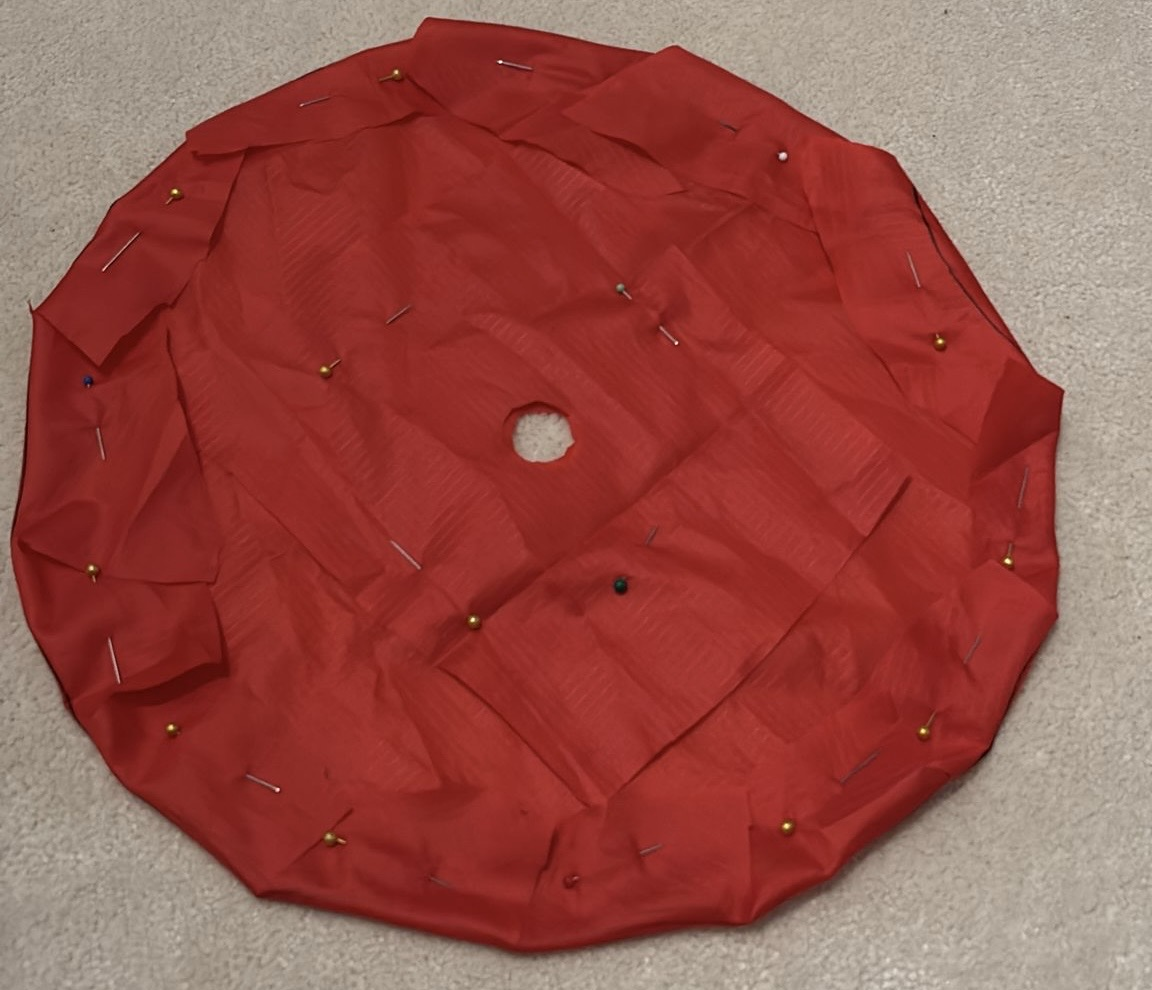
\includegraphics[width=0.4\textwidth]{images/Screen_parachute.jpg} 
    \caption{Parachute in construction}
\end{figure}

\subsubsection{Can}

The can is quite advanced but it is not our final model. We still need to optimize the space. Our design
respects the requirements of a 66mm diameter and a height of 115mm. We have a hole for the Airtag and 2
compartments. One will contain the BMP280 and the radio module and the second one will contain the charger
and the battery. We believe that our can is ergonomic. The Figure 2 shows what it looks like. 

\begin{figure}[h]
    \centering
    \subfloat{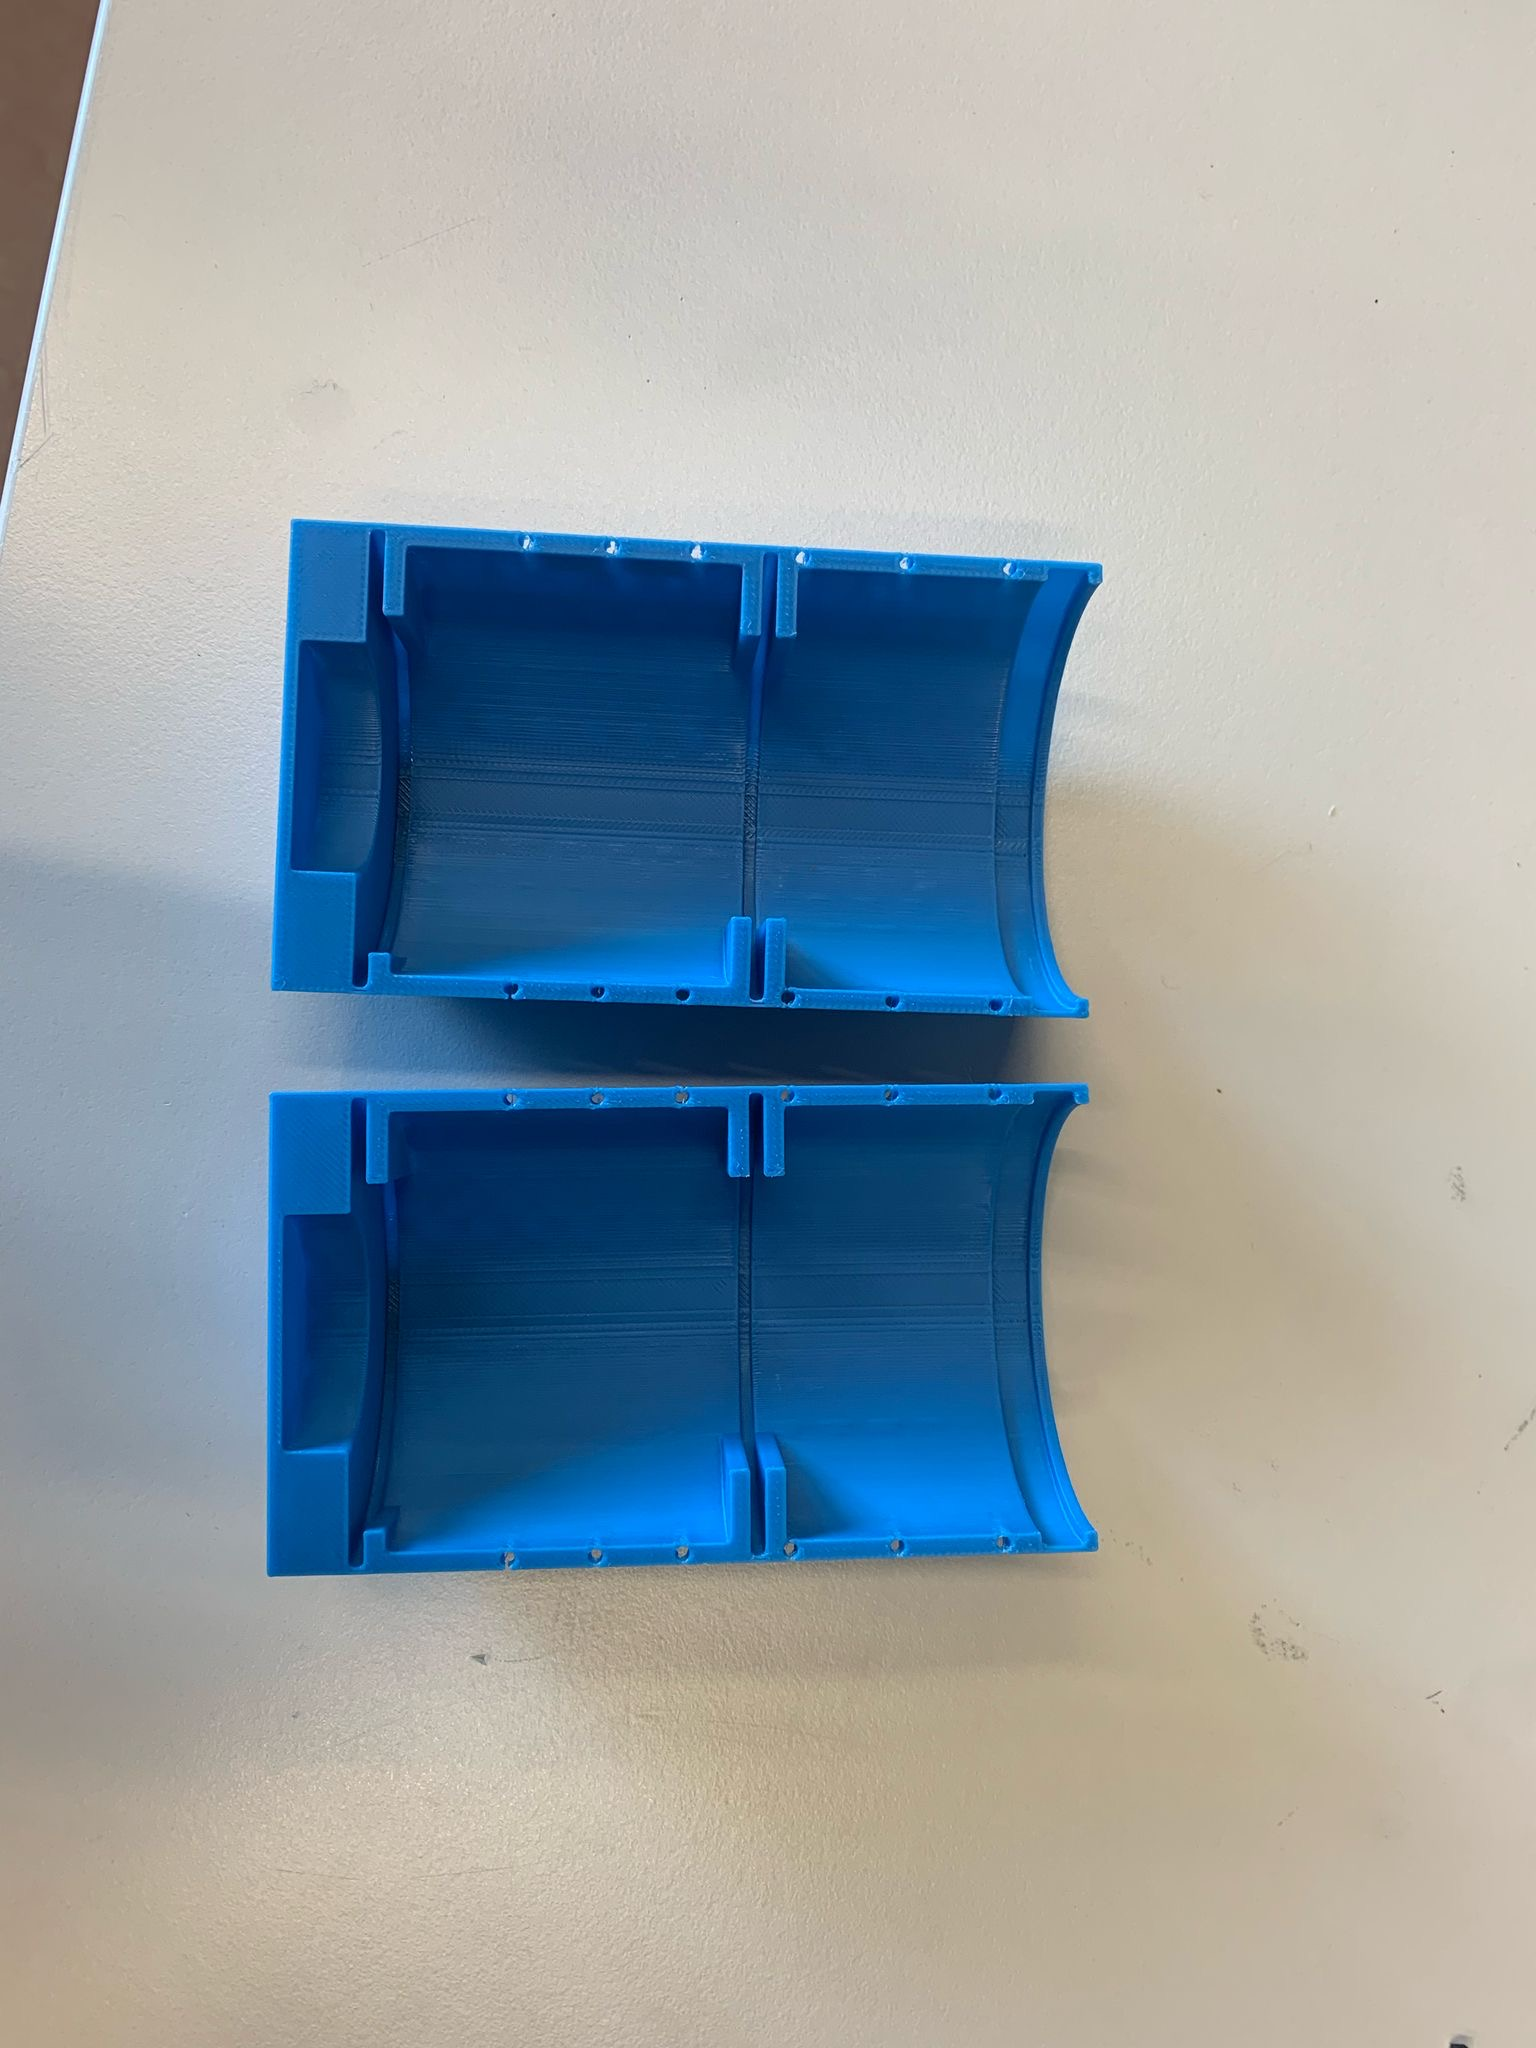
\includegraphics[width=0.3\textwidth]{images/Photo_canbleue.JPG}}
    \hfill
    \subfloat{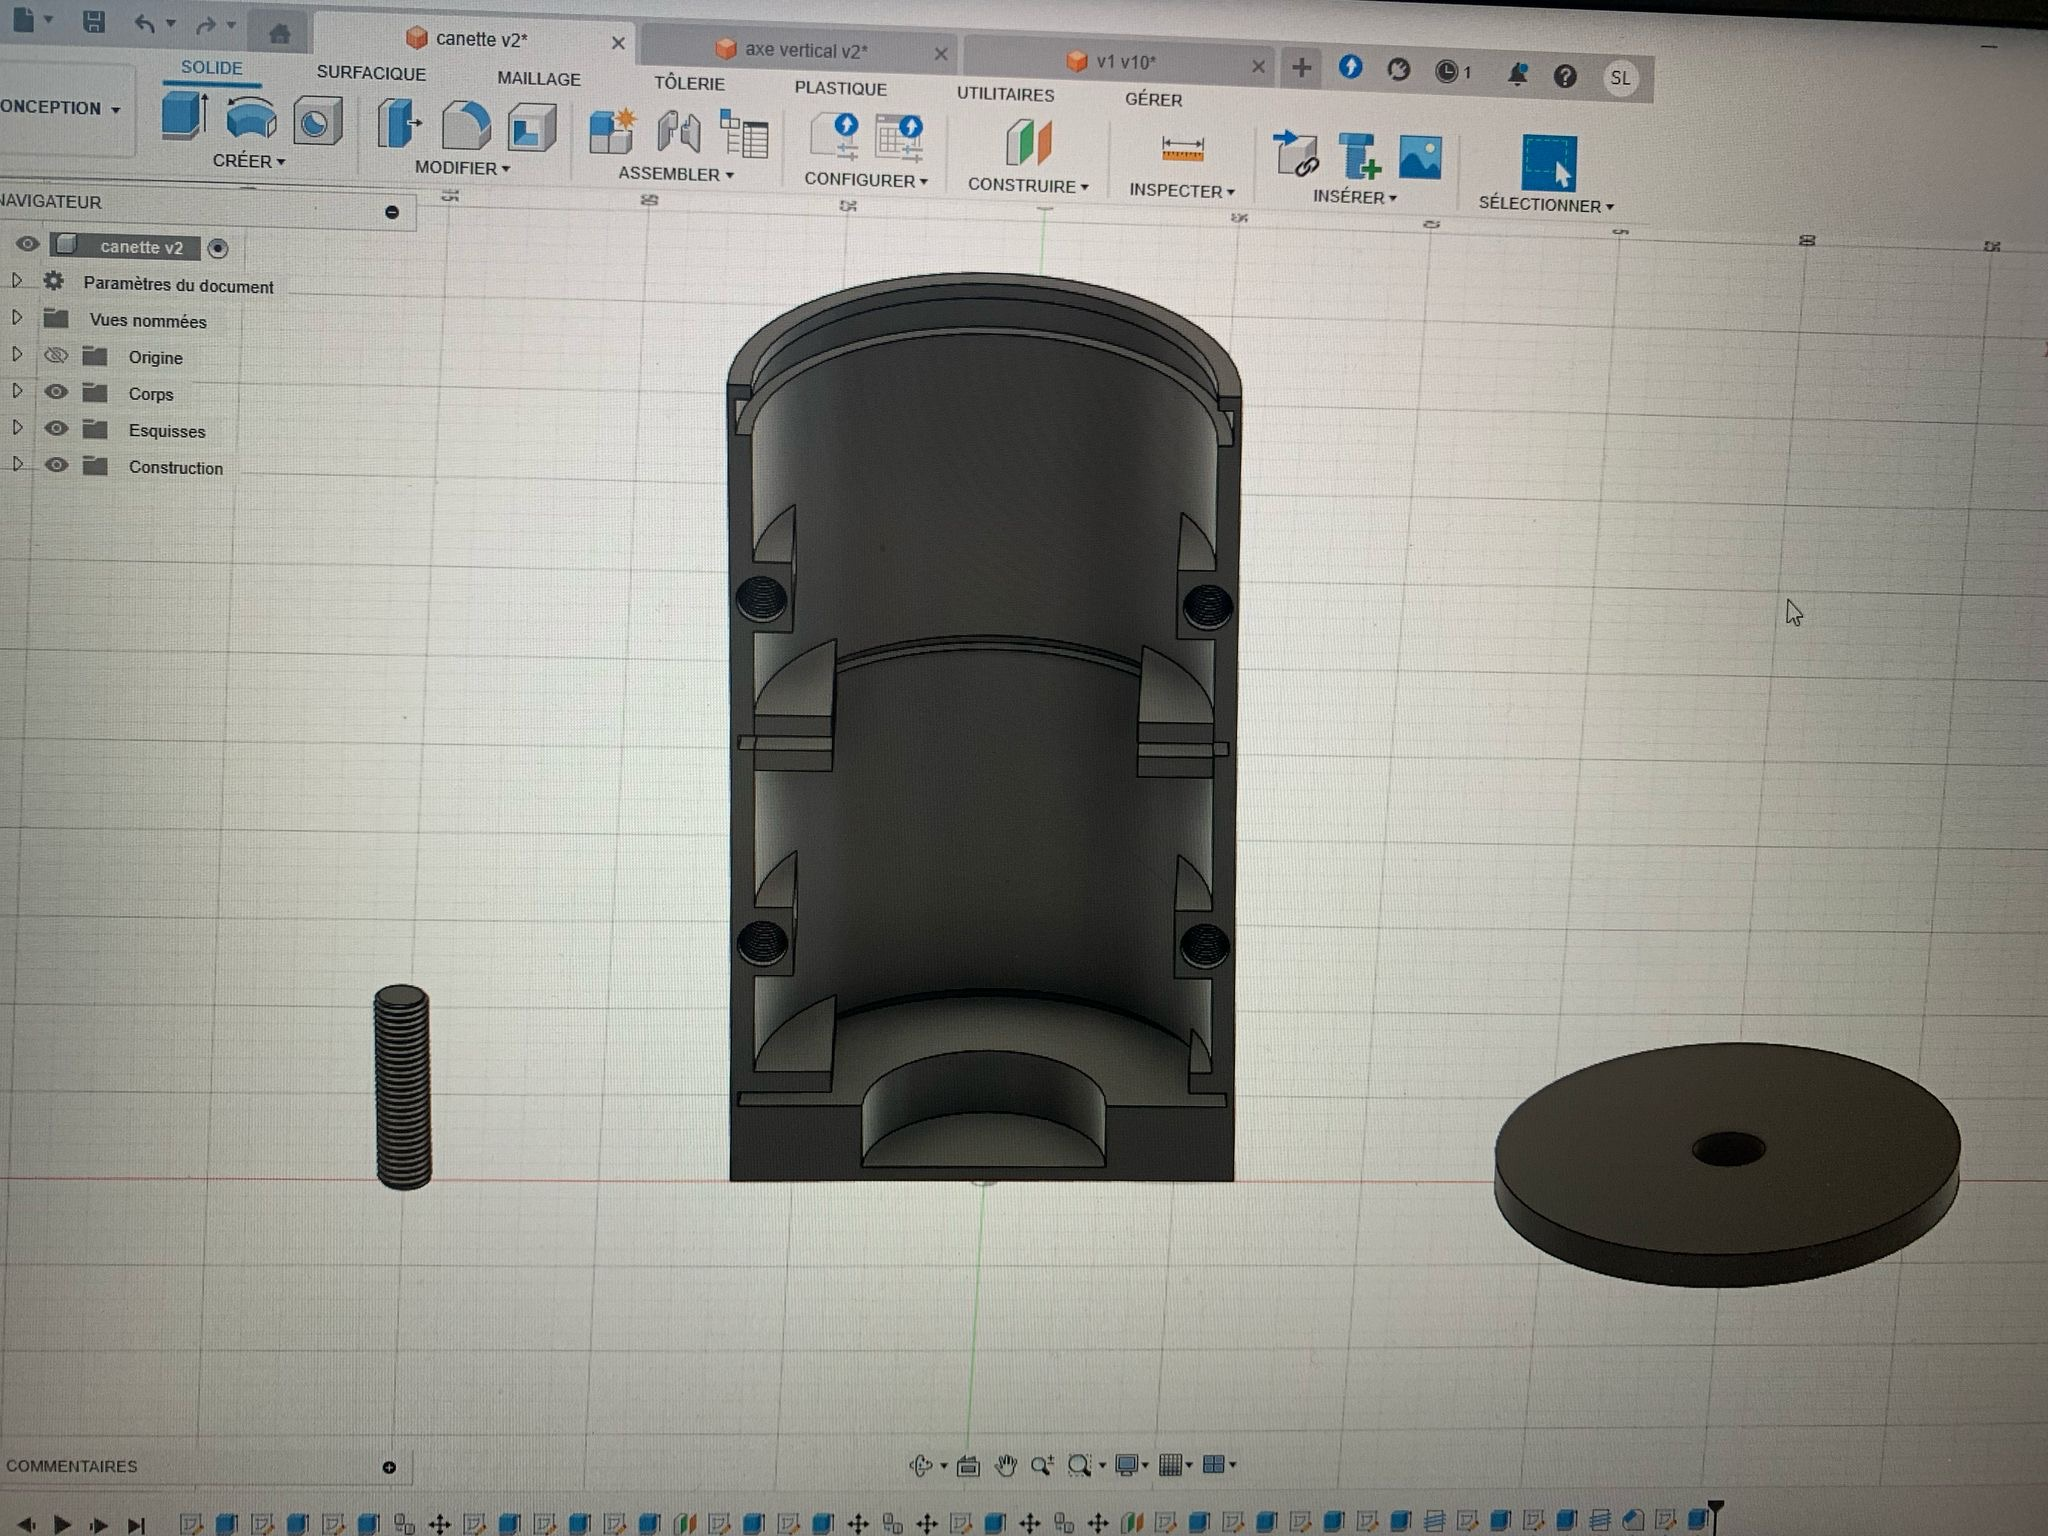
\includegraphics[width=0.5\textwidth]{images/Schema_canfinale.JPG}}
    \caption{Our can}
\end{figure}


\subsubsection{Tracking}

The tracking system (Figure 3) is rather good so far. Our vertcal axis is good as we have the clamp. We also have
the horizontal axis but it needs to be perfected and we cannot test it yet because it depends on the 
vertical axis. So, the only completely functionning item of the tracking is the clamp.

\begin{figure}[h]
    \centering
    \subfloat{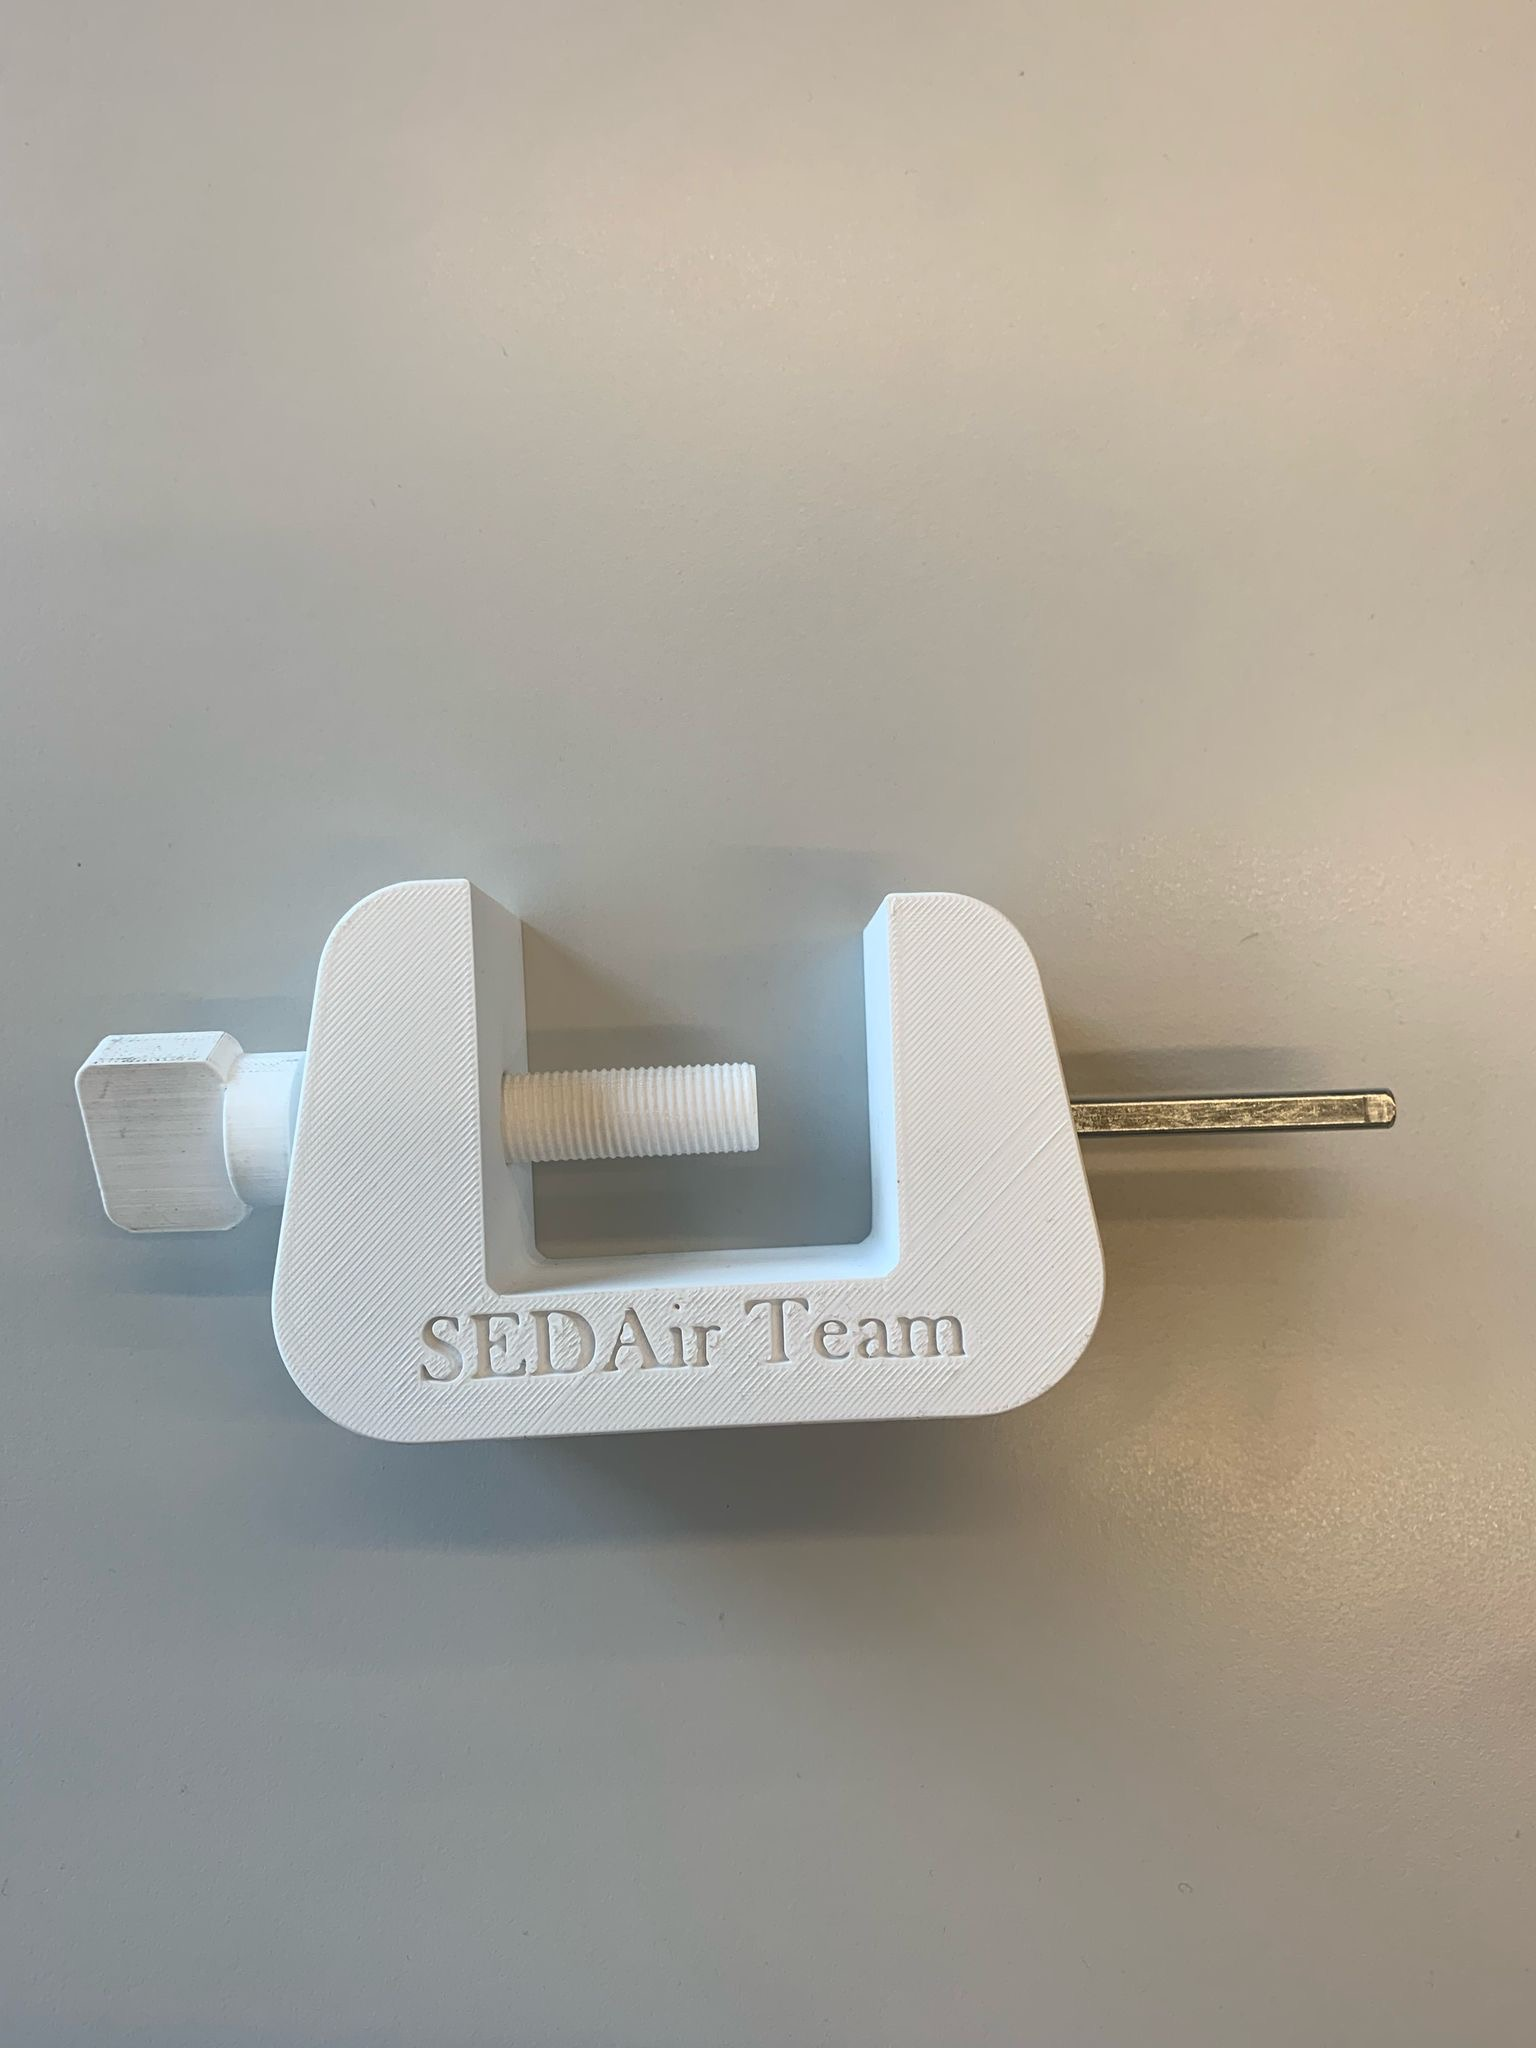
\includegraphics[width=0.3\textwidth]{images/Photo_clamp.JPG}}
    \hfill
    \subfloat{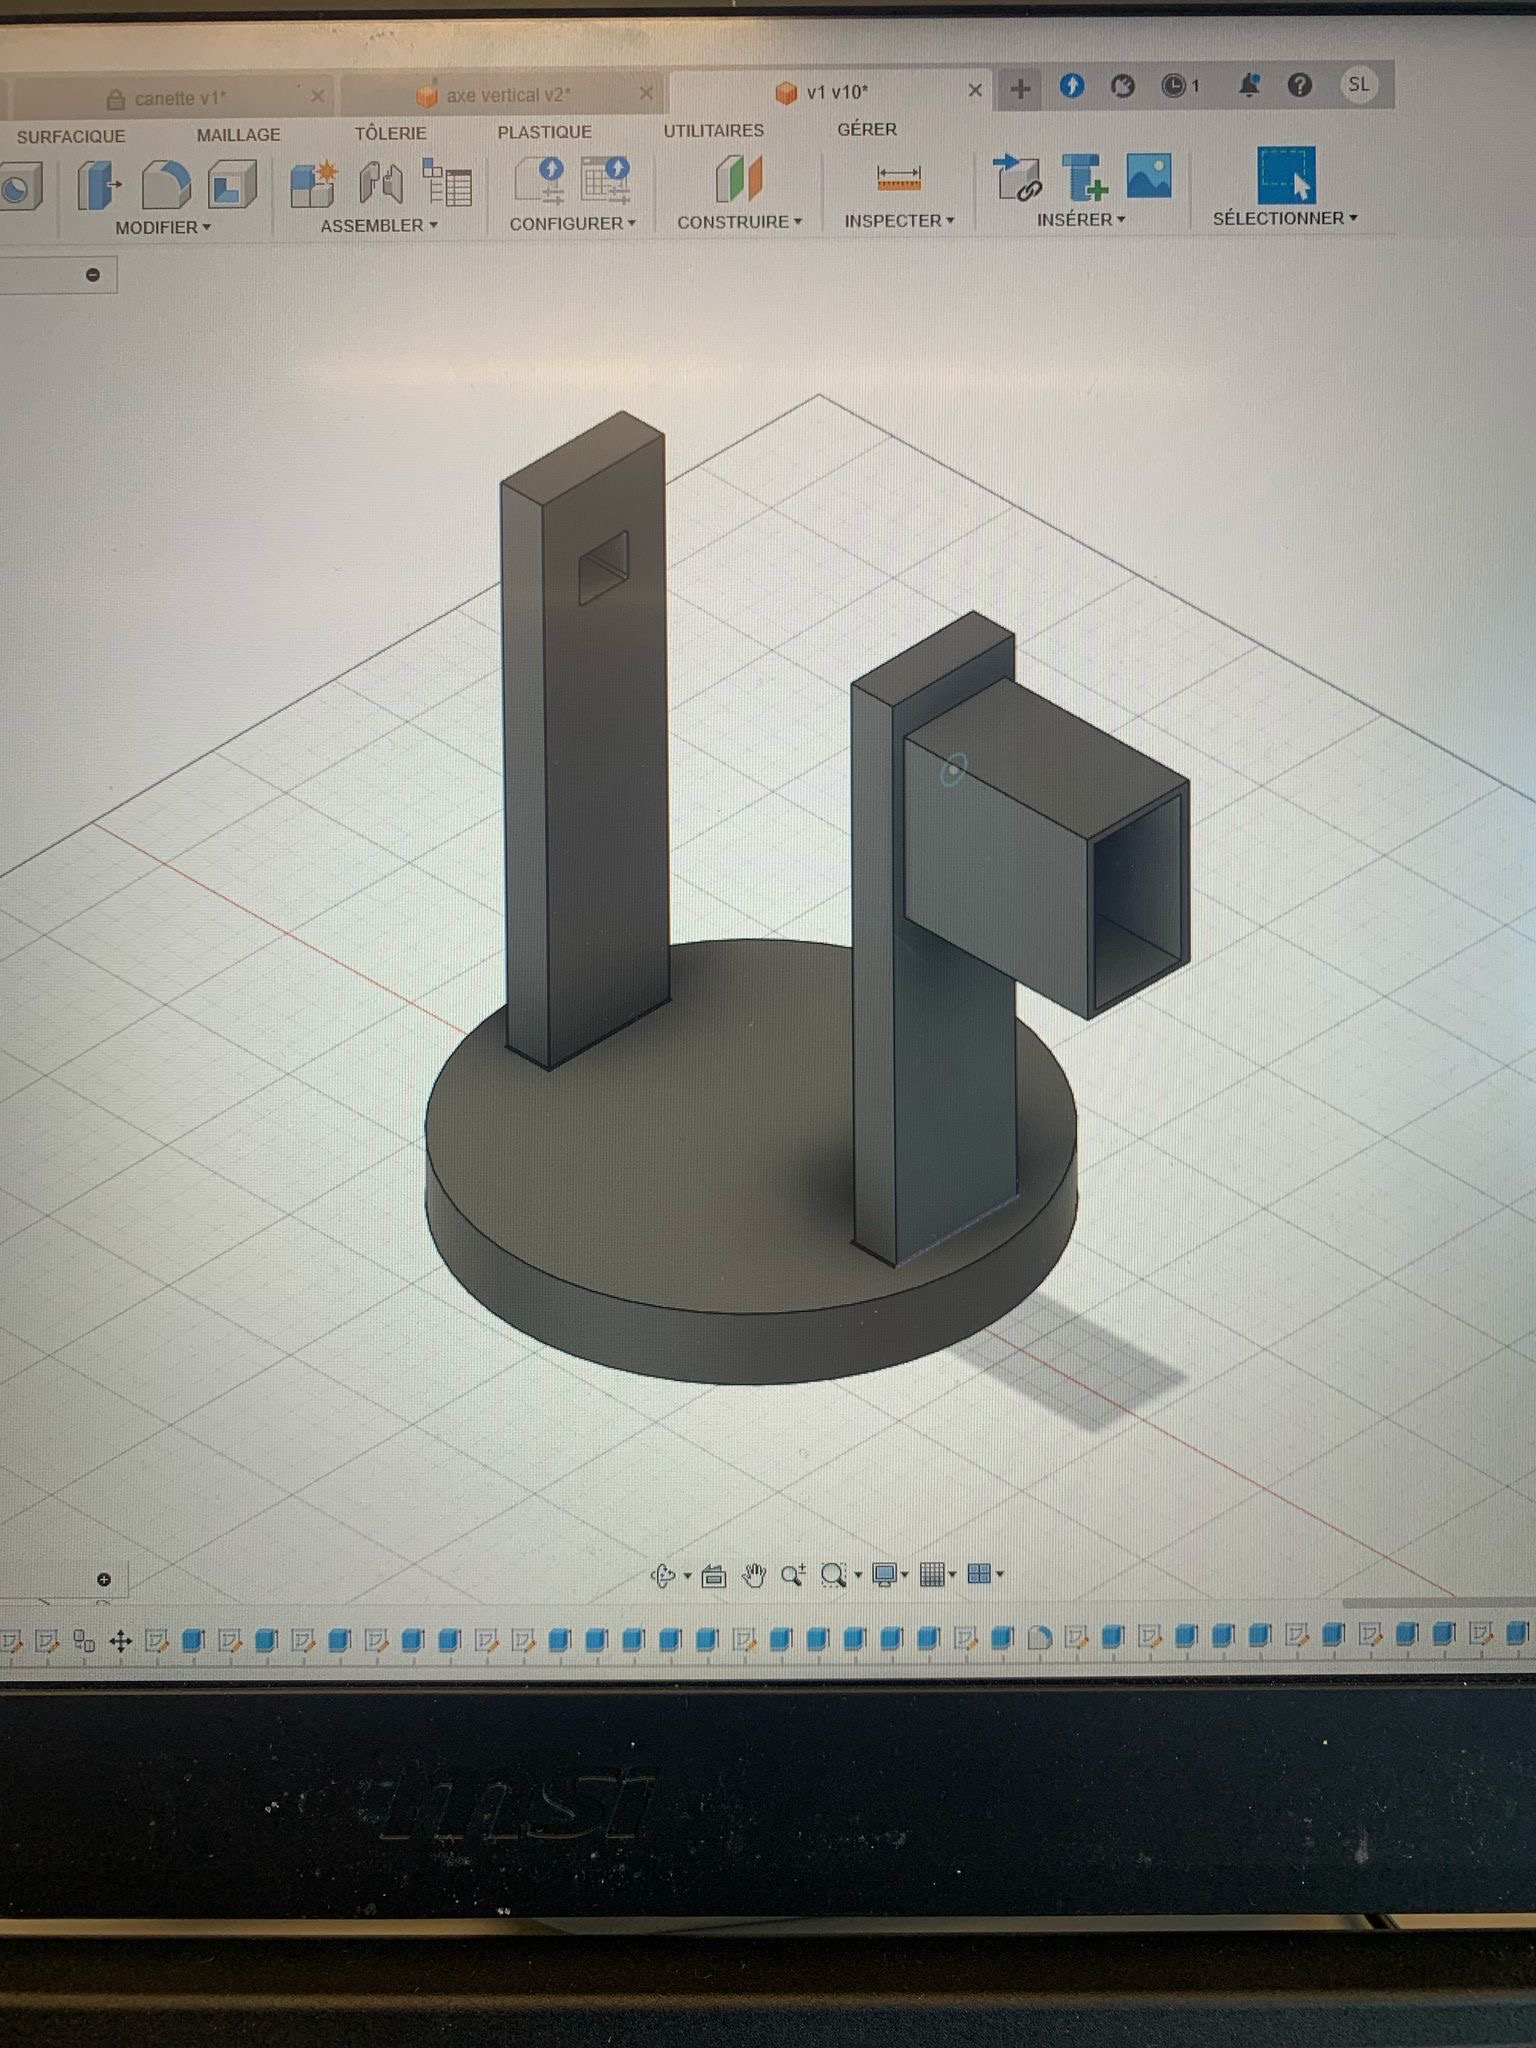
\includegraphics[width=0.3\textwidth]{images/3D_vertical.JPG}}
    \hfill
    \subfloat{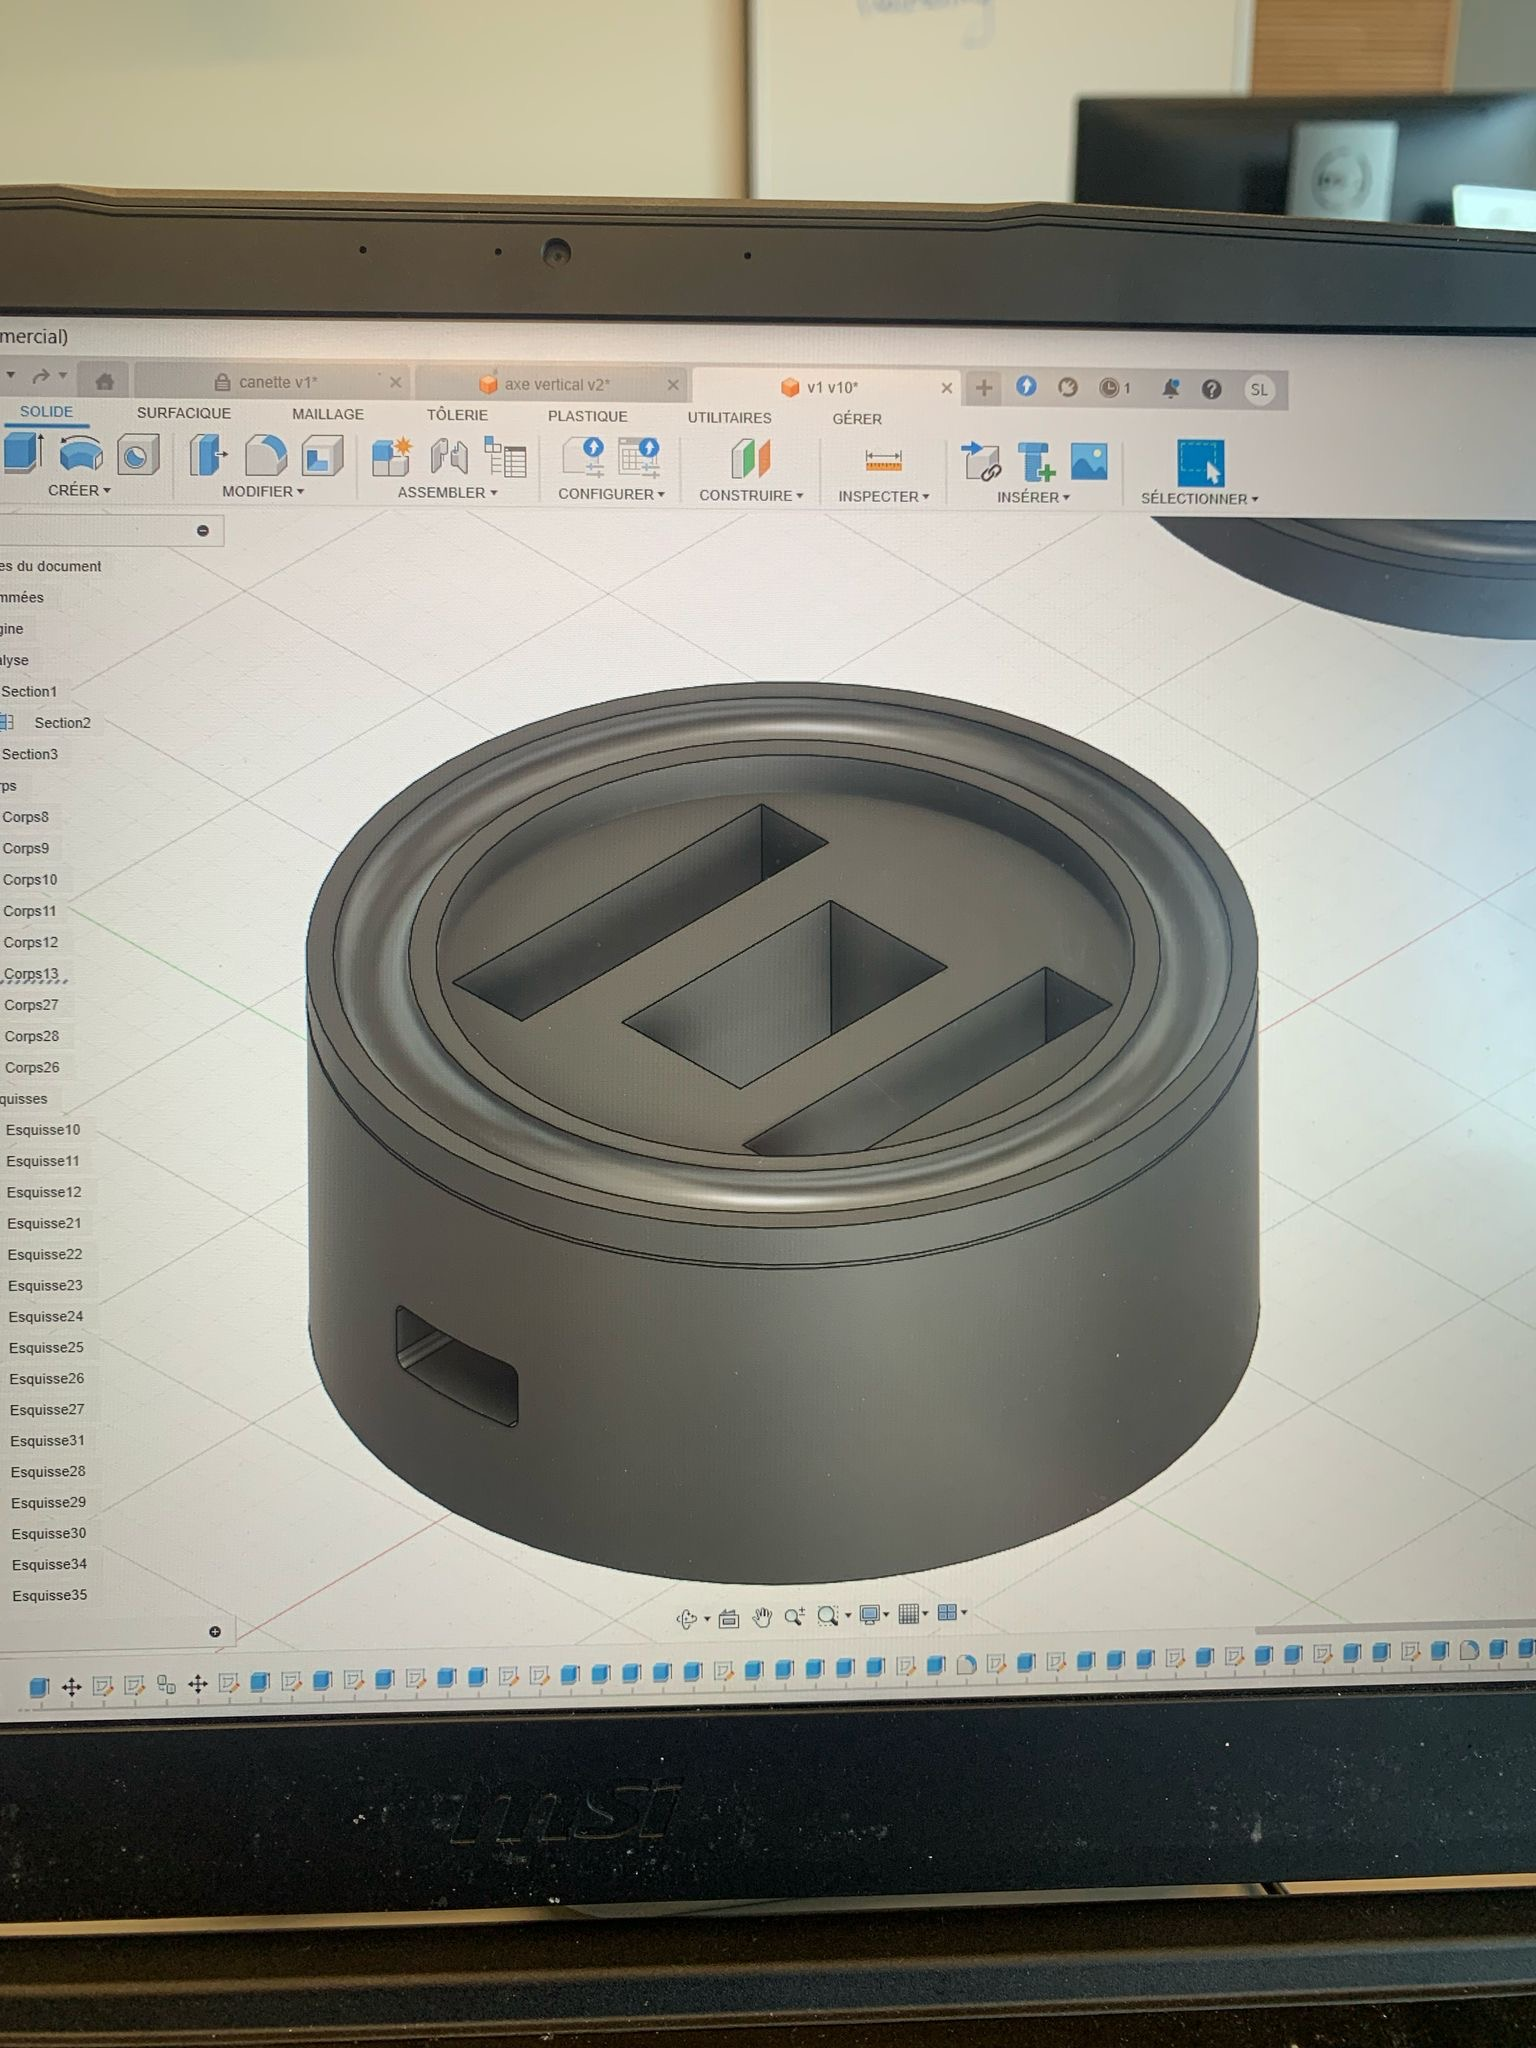
\includegraphics[width=0.3\textwidth]{images/3D_horizontal.JPG}}
    \caption{The components of our tracking system (clamp, vertical axis, horizontal axis)}
\end{figure}

\newpage

Eventually, the tracking should look like this (Figure 4): 

\begin{figure}[h] 
    \centering
    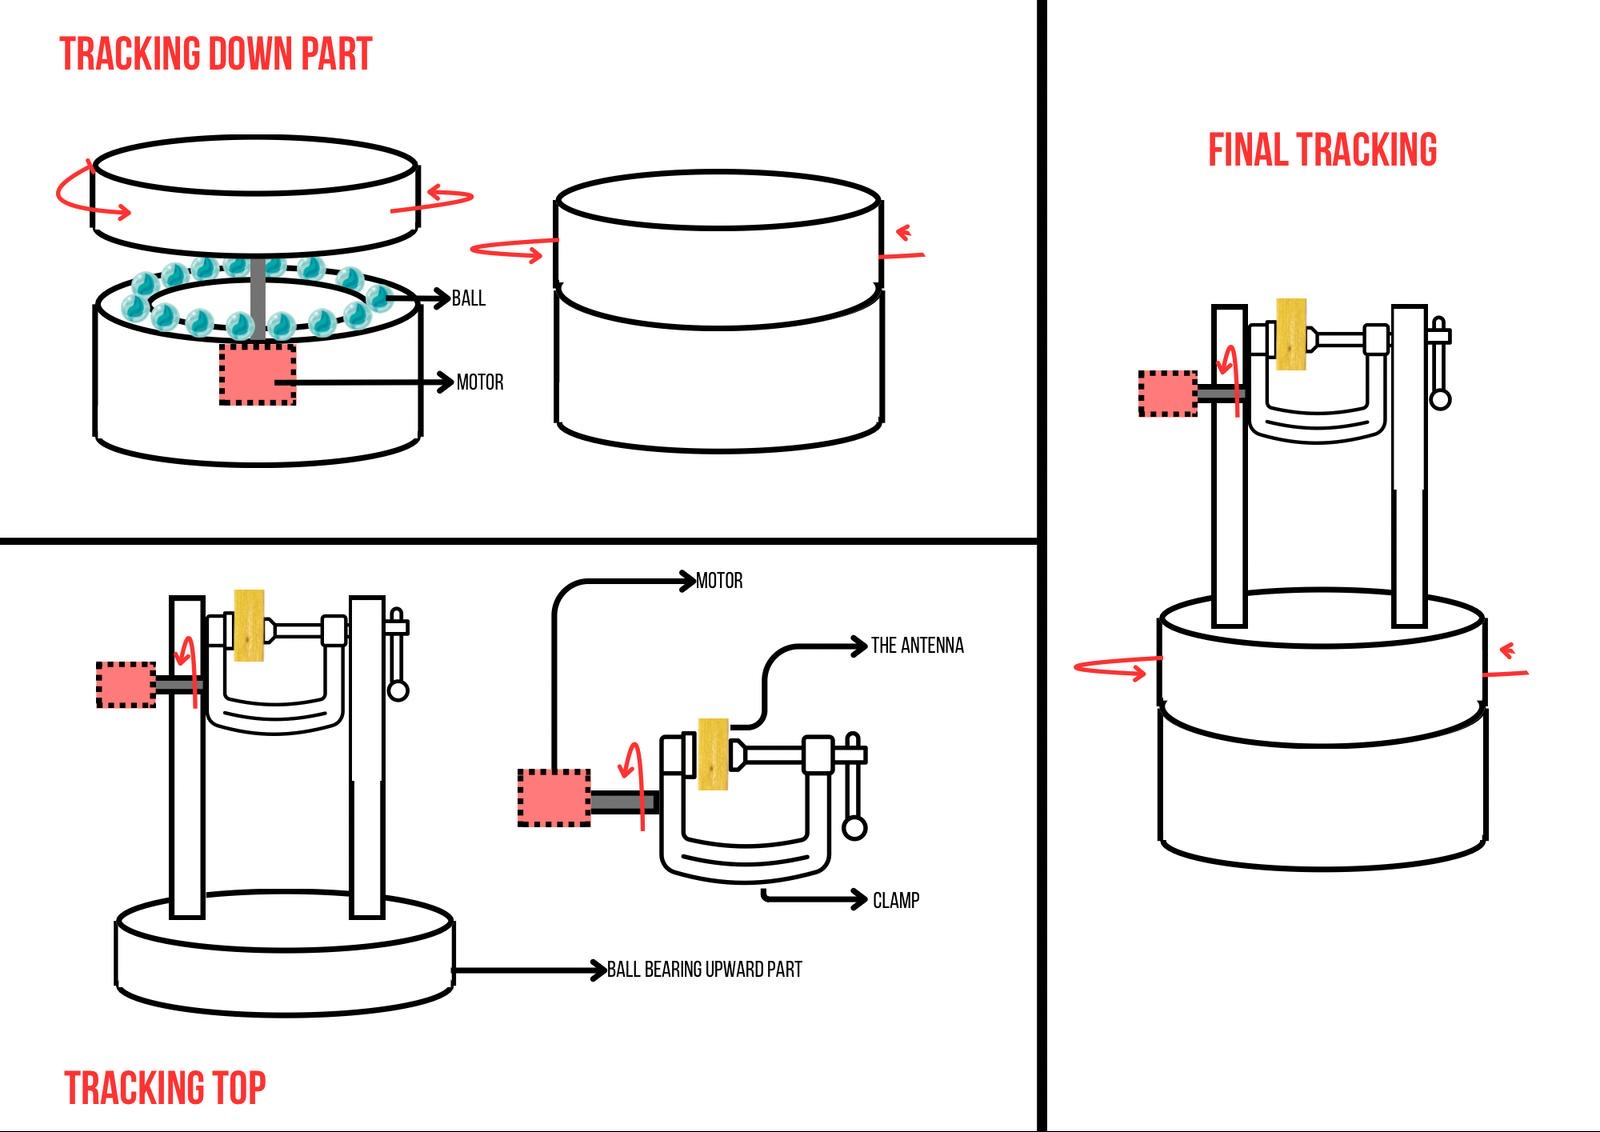
\includegraphics[width=0.5\textwidth]{images/Schema_trackingcomplet.JPG} 
    \caption{Finished tracking system}
\end{figure}

\subsection{Electronic design}

\subsubsection{Emitter - PCB}

Our emitter is soldered on a PCB, just like in the Figure 5. The BMP280, RFM69 and the lipo boost charger
are very easy to code and give great results, that's why we chose to use them and it works very well. We used the wiring
on the McHobby website so our electronic design is not quite special or innovative (Figure 6). 

\begin{figure}[h] 
    \centering
    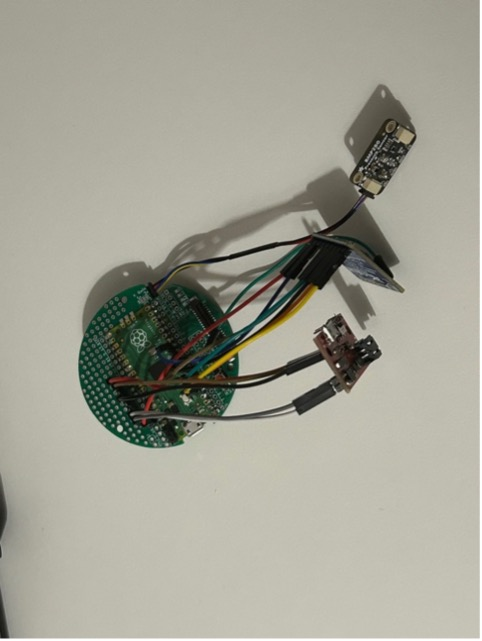
\includegraphics[width=0.3\textwidth]{images/photo_soldering.jpg} 
    \caption{Soldered PCB}
\end{figure}

\vspace{2em}

\begin{figure}[h]
    \centering
    \subfloat{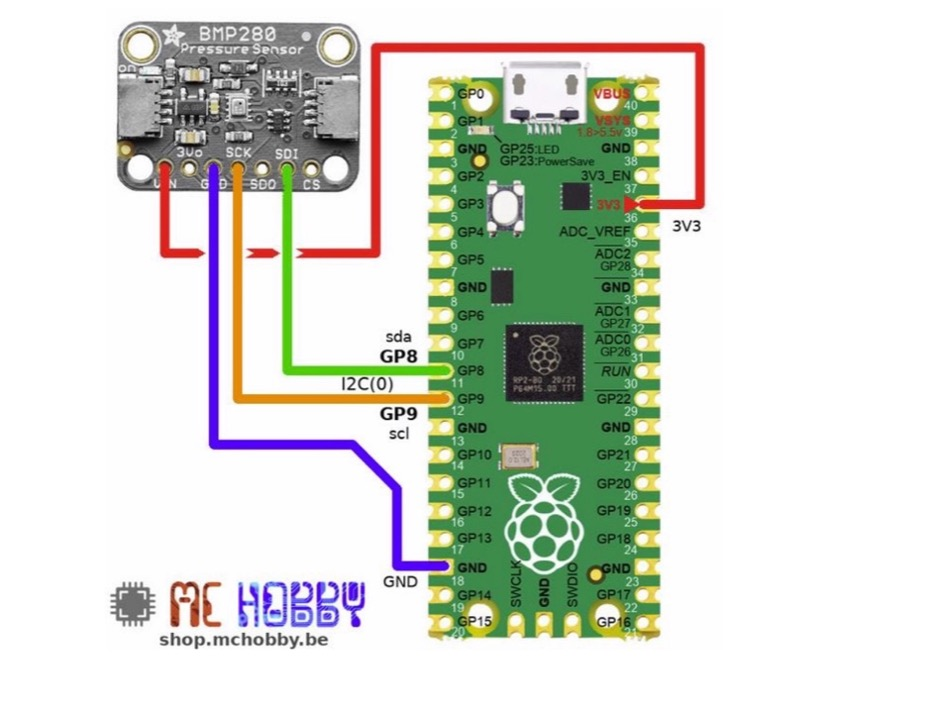
\includegraphics[width=0.3\textwidth]{images/schema_bmpconnexion.jpg}}
    \hfill
    \subfloat{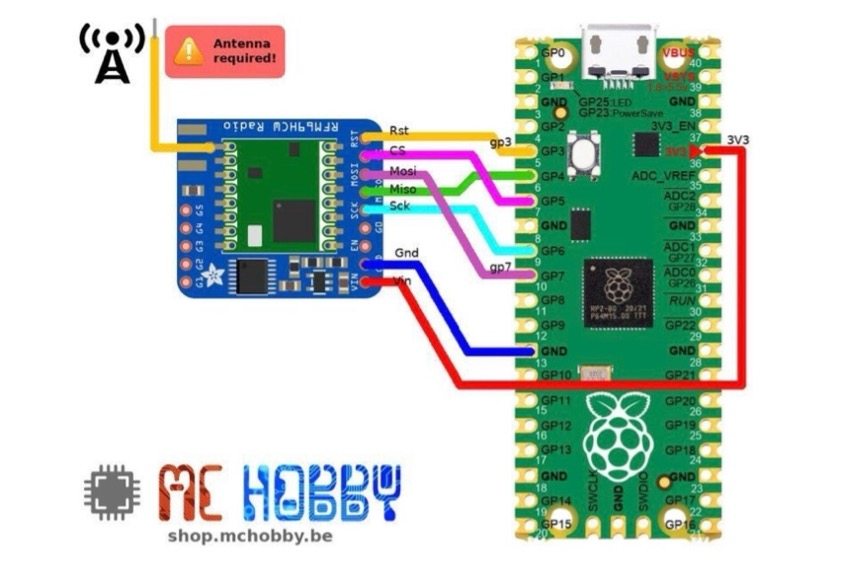
\includegraphics[width=0.3\textwidth]{images/schema_rfmconnexion.jpg}}
    \hfill
    \subfloat{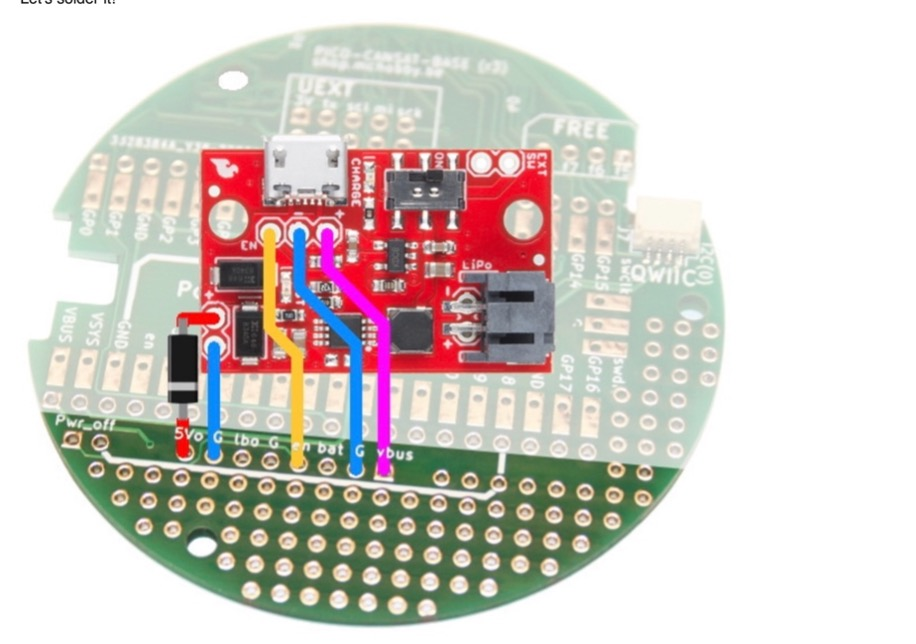
\includegraphics[width=0.3\textwidth]{images/schema_batteryconnexion.jpg}}
    \caption{The electronic design in our CanSat}
\end{figure}


\subsubsection{Receiver - Ground station}

The ground station does not have something special or innovative, we used the wiring given on the
McHobby website and the data is received with the RFM69 connected to a raspberry pi pico on a breadboard (Figure 7).

\begin{figure}[h] 
    \centering
    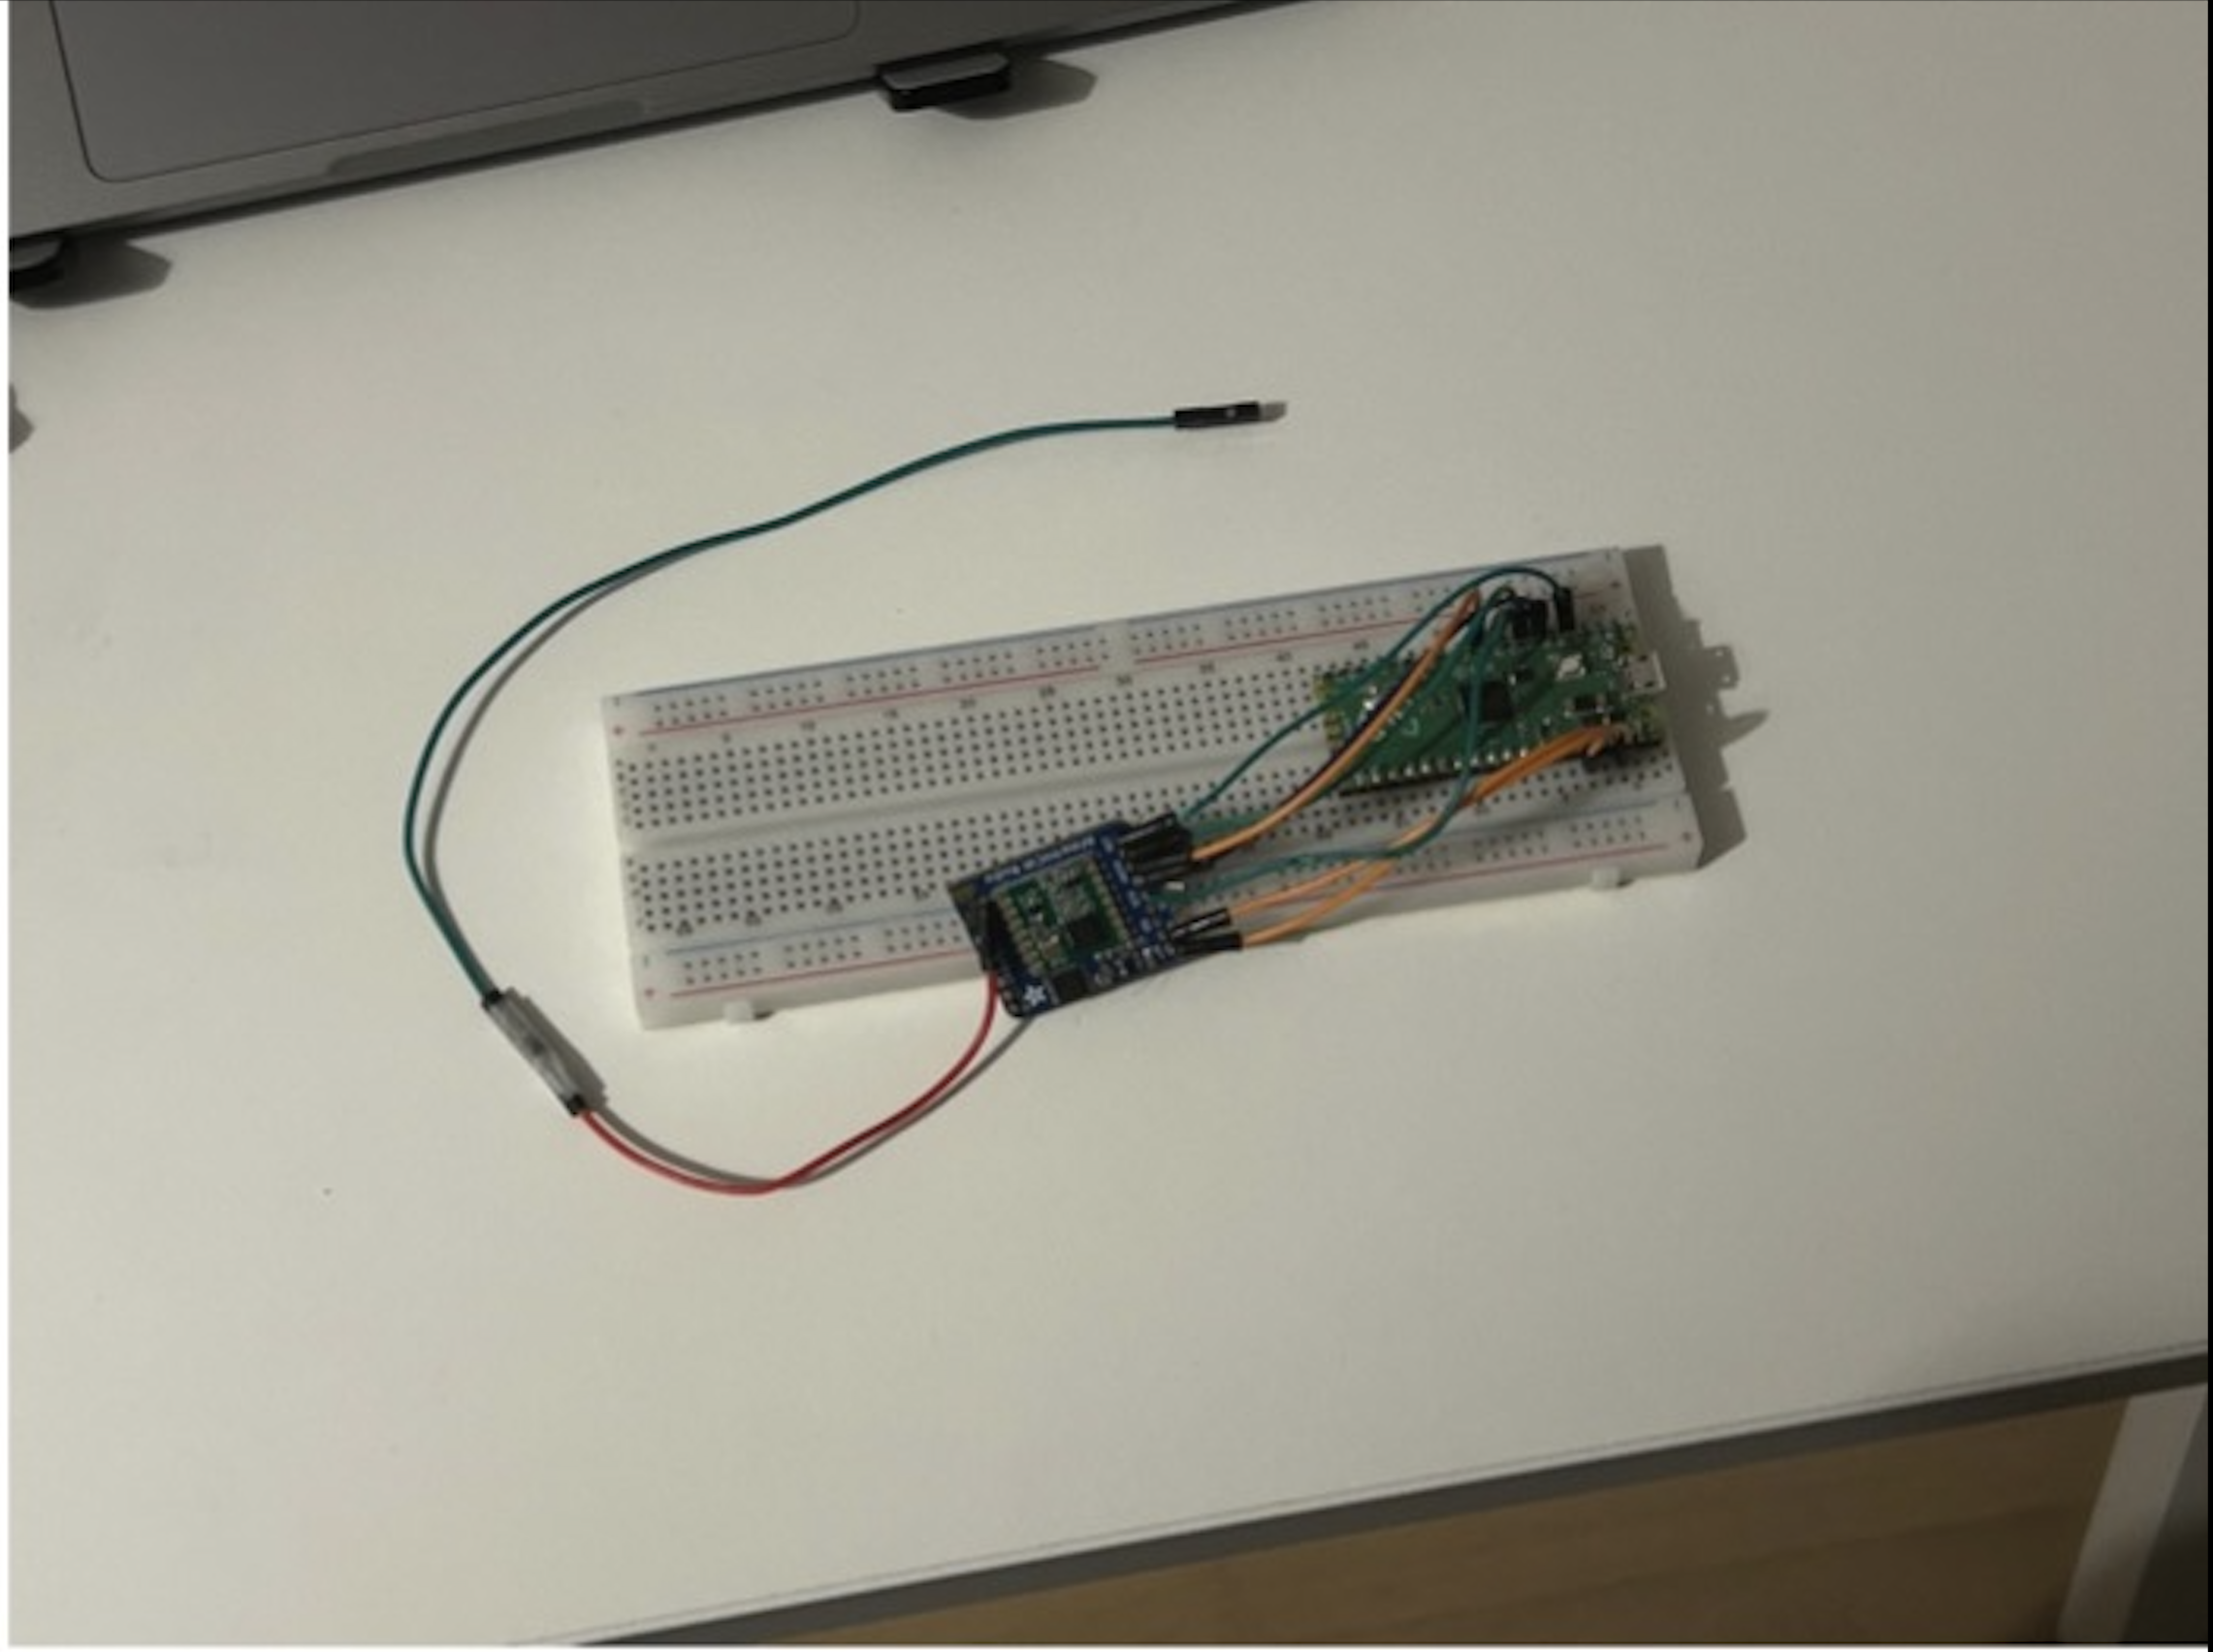
\includegraphics[width=0.3\textwidth]{images/photo_groundstation.png} 
    \caption{Ground station}
\end{figure}

\subsection{Ground station design}

The photo of our ground station was in part \textbf{2.3.2}. It is connected to our antenna with a coaxial cable and to 
a computer to run the code and get the values. The ground station stores the values it receives in the flash memory of the 
raspberry pi pico. With our secondary mission, the tracking should be part of it but we
do not have any photo to provide yet. 

\subsection{Software design}
\subsubsection{Emitter code}

The message (variable "msg") that sends our emitter is structured as follows : 

\begin{itemize}[left=4em]
    \item iteration index
    \item time in seconds
    \item pressure
    \item temperature
    \item altitude
\end{itemize}

Our emitter's algorithm is very basic. The Figure 8 shows the structure. 

\begin{figure}[h] 
    \centering
    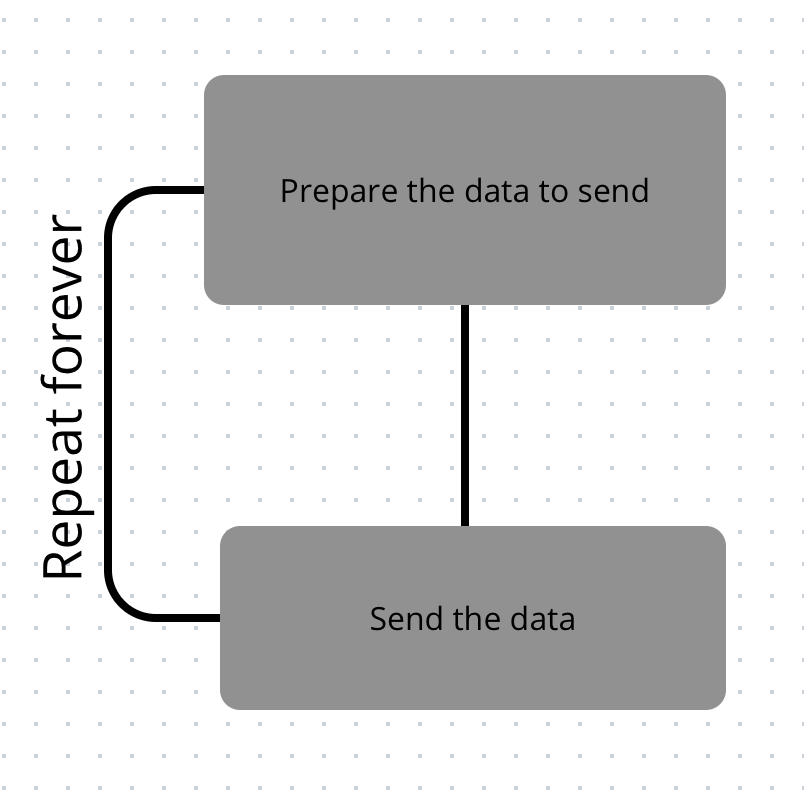
\includegraphics[width=0.26\textwidth]{images/emitter_diagram.png} 
    \caption{Emitter flowchart}
\end{figure}

\subsubsection{Receiver code}

The receiver receives the variable "msg" in a little different algorithm (Figure 9).

\begin{figure}[h] 
    \centering
    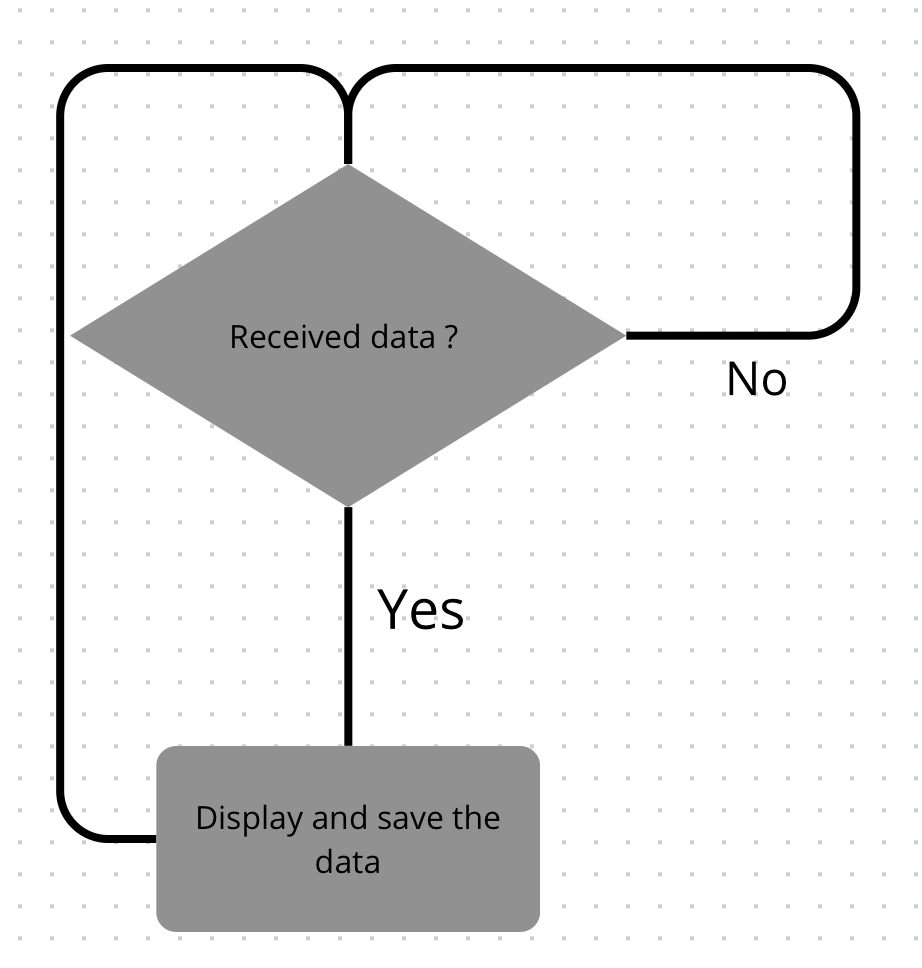
\includegraphics[width=0.26\textwidth]{images/receiver_diagram.png} 
    \caption{Receiver flowchart}
\end{figure}


\newpage
\subsubsection{Quantitative analysis code}

Our quantitative analysis program plots our data in different graphs and gives the maximum and minimum of temperature, pressure and altitude
in the set of data. You can see the results in Figure 10 and Figure 11. The set of data is completely random, it is values taken at home. 

\begin{figure}[h]
    \centering
    \subfloat{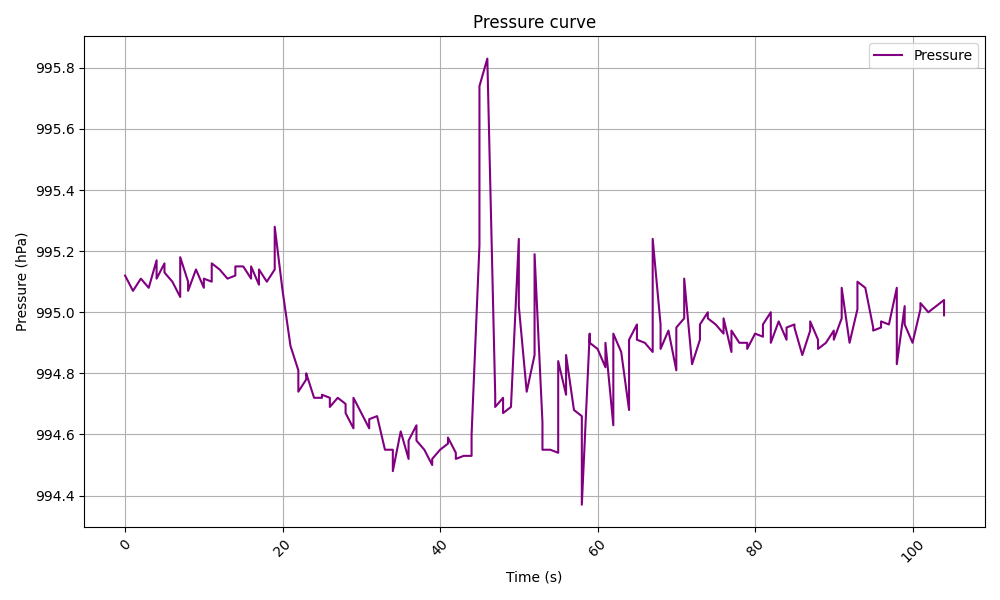
\includegraphics[width=0.3\textwidth]{images/quantpressure.png}}
    \hfill
    \subfloat{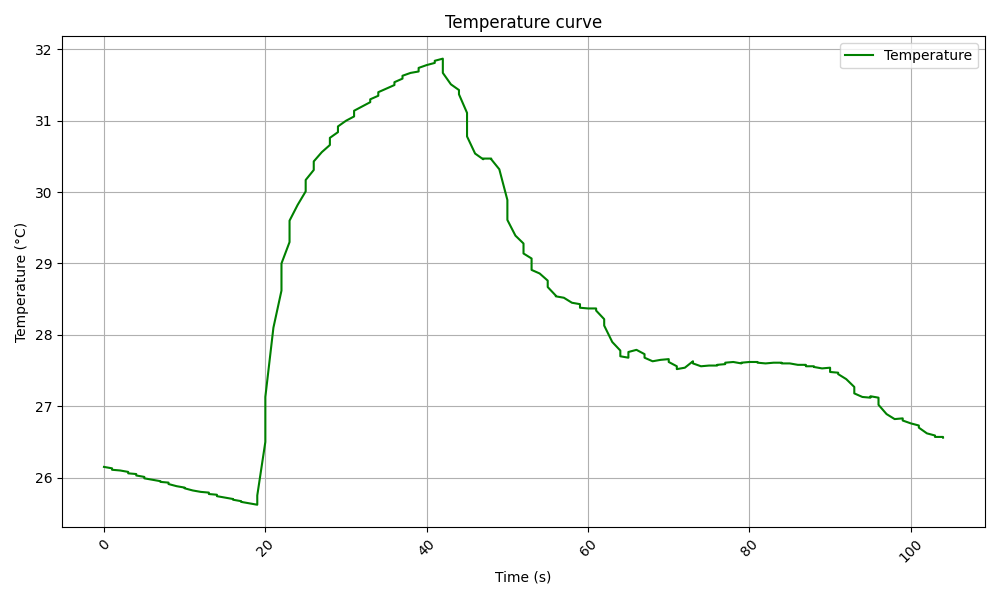
\includegraphics[width=0.3\textwidth]{images/quanttemp.png}}
    \hfill
    \subfloat{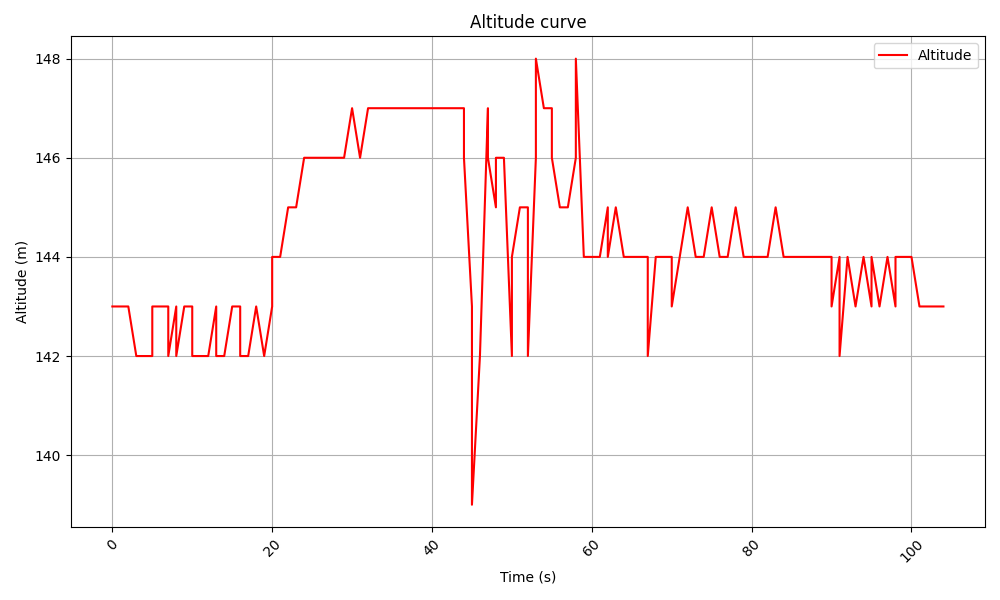
\includegraphics[width=0.3\textwidth]{images/quantalt.png}}
    \caption{Graphs of our data}
\end{figure}

\begin{figure}[h] 
    \centering
    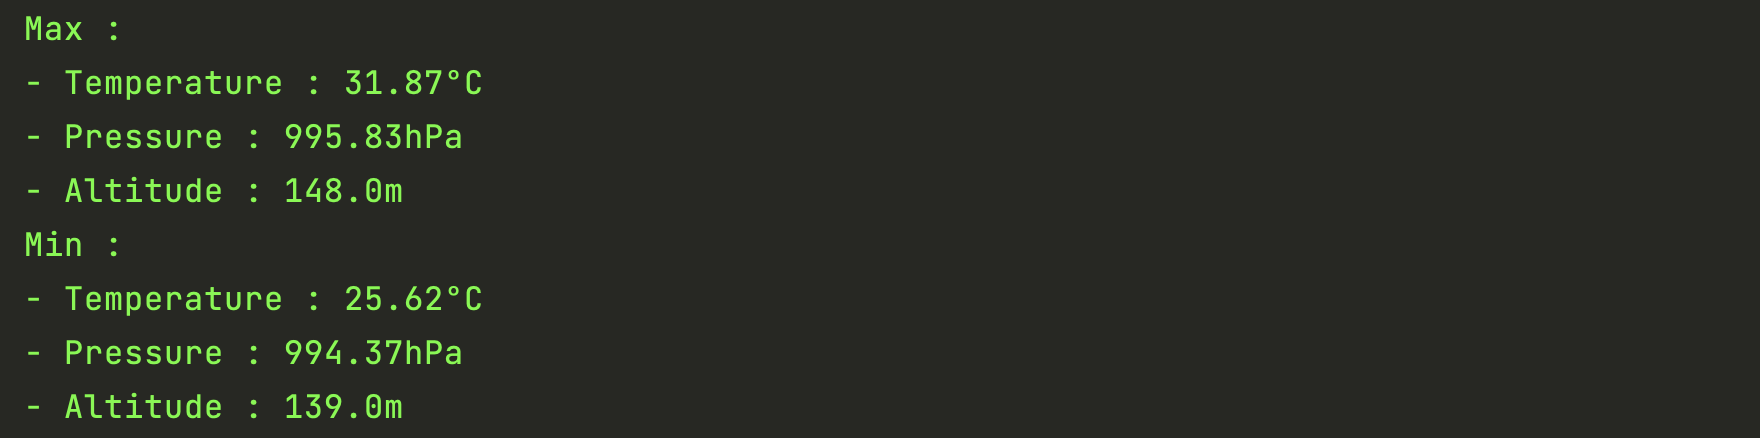
\includegraphics[width=0.6\textwidth]{images/quantdata.png} 
    \caption{Min-Max in the analysis}
\end{figure}

\subsection{Recovery system}

\subsubsection{Airtag}

To recover our CanSat, of course we will use our parachute, but we already described it earlier.
We will try to use an AirTag (Figure 12) that works with our phone. You told us that it does not work, so we will
test it first and then we will work on another system. 

\begin{figure}[h] 
    \centering
    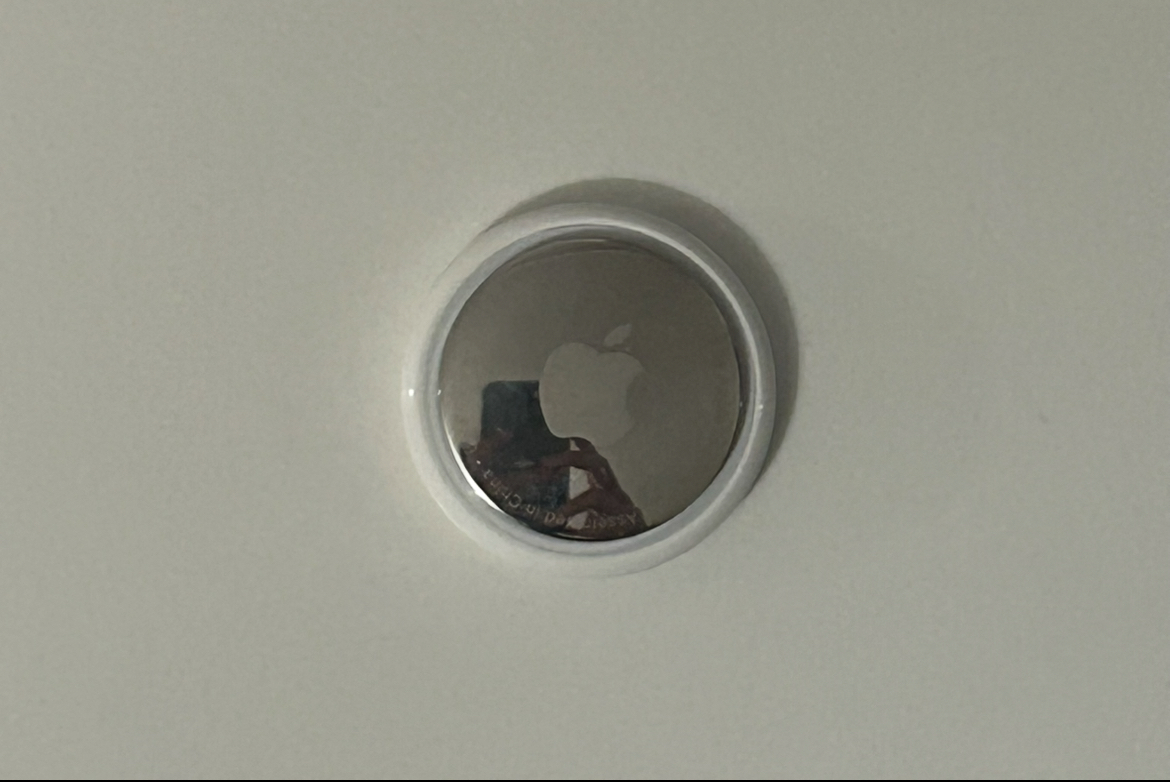
\includegraphics[width=0.3\textwidth]{images/Airtag .jpg} 
    \caption{Airtag}
\end{figure}

\subsubsection{Buzzer}

We do not have a buzzer yet, so we did not work on it. But we will try to code a buzzer
to recover our CanSat instead of the AirTag. Thank you for telling us that the AirTag is risky.

\subsection{Testing}

What are the tests we did :
\begin{itemize}
    \item Primary mission at home - Working
    \item Primary mission with the antenna (200m distance) - Working
    \item Quantitative analysis program - Working 
\end{itemize}

According to our calculations, our CanSat can store data for up to 7h becaus 1 seconds of data costs 74.2kB of Flash memory
and we have 1 953 700kB left after we substract the cost in memory of the code and library installed Here is an extract of 
a data file where the BMP280 felt the higher temperature (Figure 13).

\begin{figure}[h] 
    \centering
    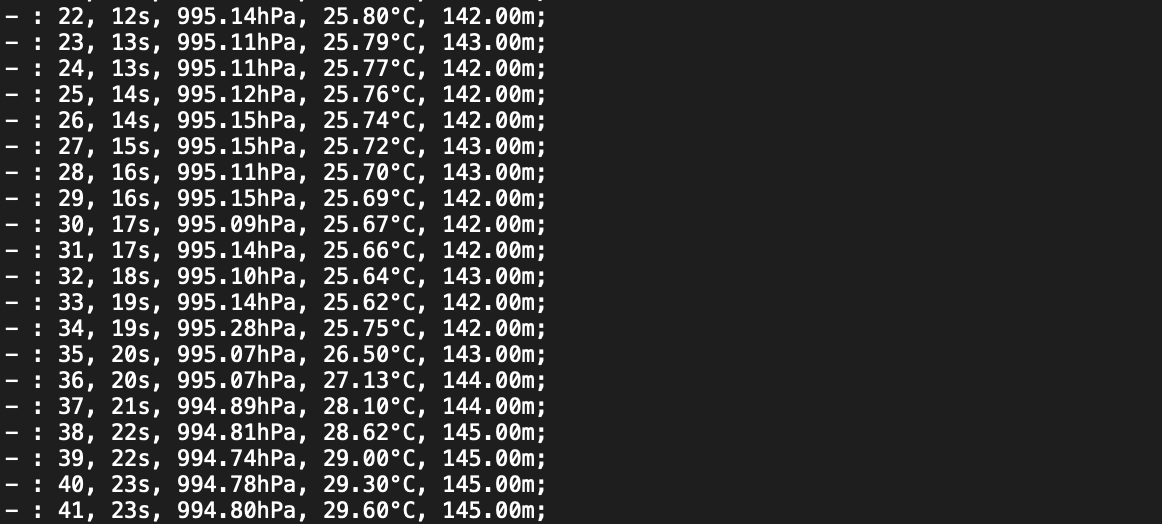
\includegraphics[width=0.6\textwidth]{images/screen_scientificresults.png} 
    \caption{Extract of a .csv data file}
\end{figure}

What are the test we still need to do :
\begin{itemize}
    \item Print and test the Can 
    \item Print and test the tracking
\end{itemize}


%3 Requirements
\section{Requirements}

We can show how we tick every requirements in the table below. 

\begin{center}
    \begin{tabular}{|c|c|} % 'c' pour centrer les colonnes, '|' pour les lignes verticales
        \hline % Ligne horizontale
        \textbf{Requirement} & \textbf{Yes/No} \\ \hline
        Dimensions of the Can & Yes \\ \hline
        Mass of the CanSat & Yes (we will add sand in our Can) \\ \hline
        Descent Velocity & Yes (the calculations are supposed to be correct) \\ \hline
        Battery & Yes \\ \hline
        Recovery system & Yes \\ \hline
    \end{tabular}
\end{center}



%4 Overall progress
\newpage
\section{Overall progress}

\subsection{Human resources}

Samuel Labignette: he knows how to code in VEX Code blocks and how to design things in 3D with Fusion360; he oversees the whole secondary mission and he designs (and prints) the can. 

Estelle Vergeynst: she has a lot of experience in soldering; she oversees the antenna and all the soldering in our CanSat journey

Daphne Ribière: she has the most knowledge on AI among us; she oversees the the parachute (and if we have time she will code an AI algorithm for a second secondary mission)

Arthur Strimbu-Lee: he knows CanSat the best overall as he attended the competition last year, he knows very well MicroPython (and Python); he oversees the whole primary mission and the post launching analysis of the data in a Python program


\subsection{Planning}

We are satisfied of our time management, here is our planning (Figure 14). 

\begin{figure}[h] 
    \centering
    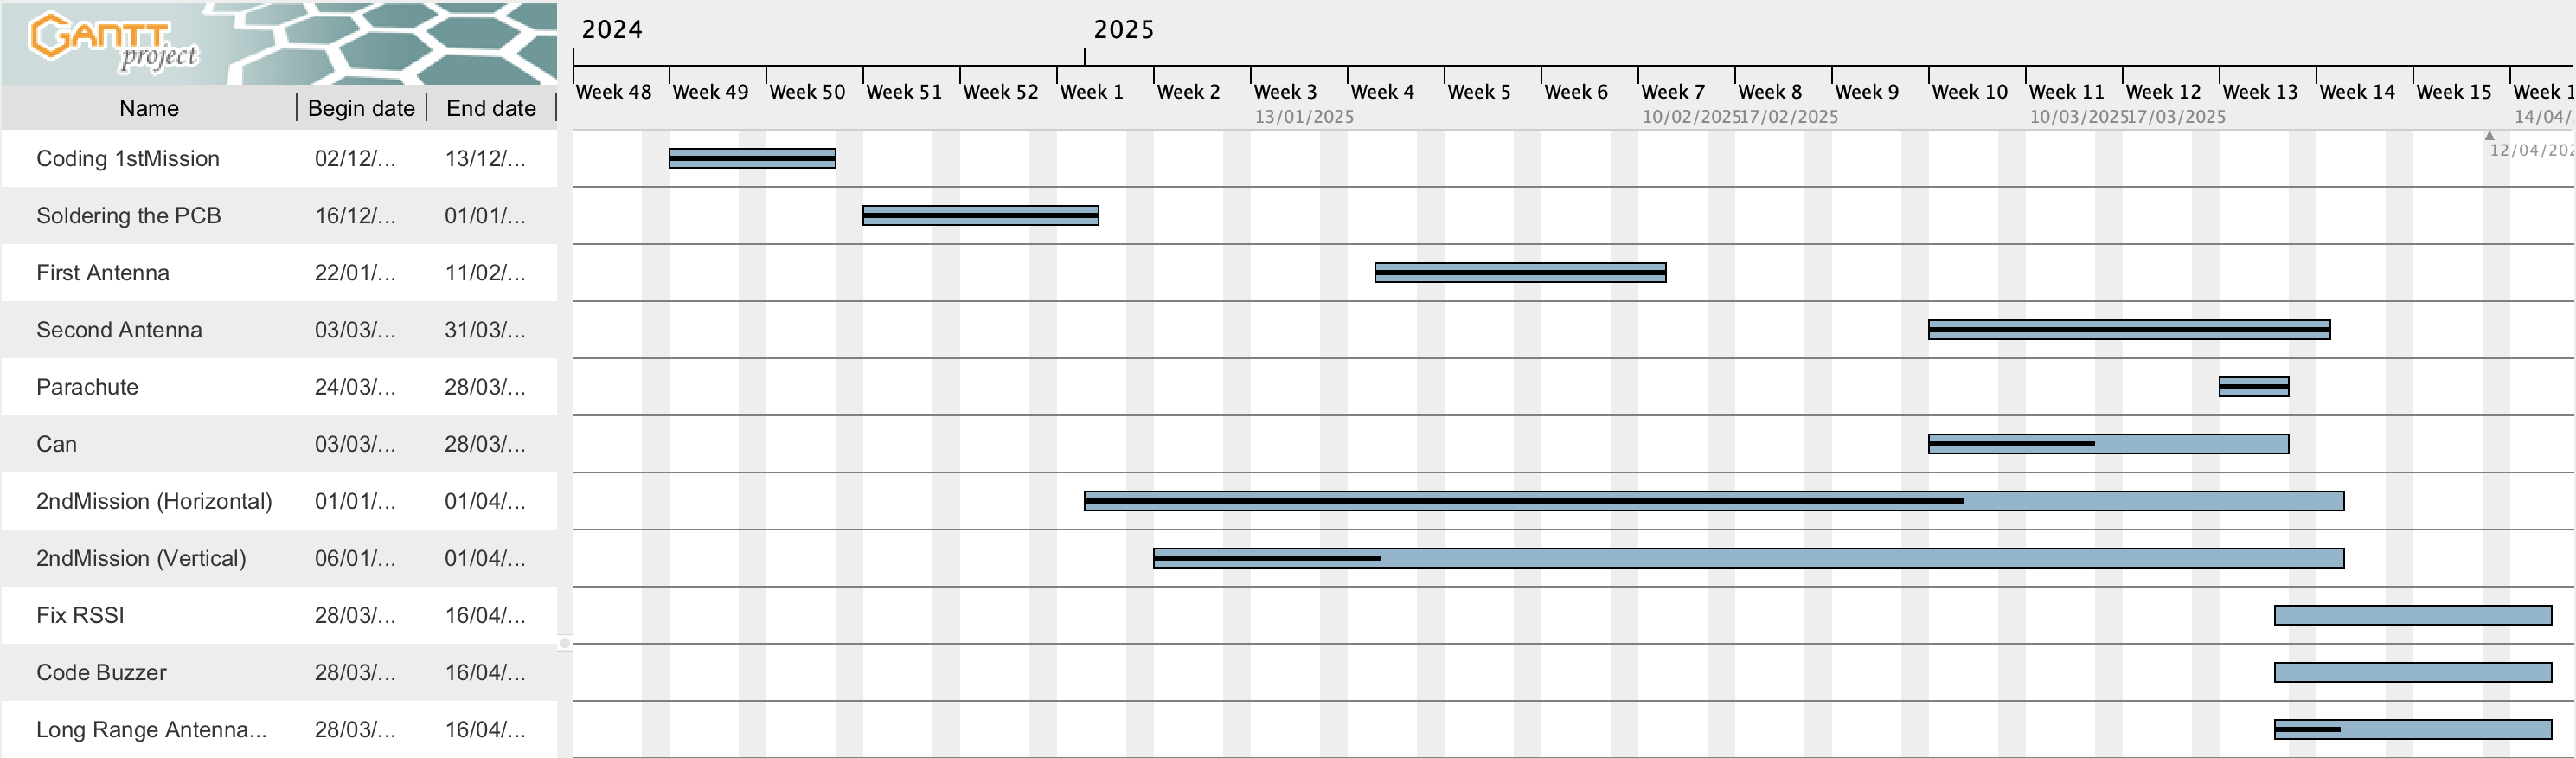
\includegraphics[width=1\textwidth]{images/planning.png} 
    \caption{Gantt Planning}
\end{figure}

\subsection{Budget}

\begin{center}
    \begin{tabular}{|l|c|}
        \hline
        \textbf{Object or 3D printing} & \textbf{Price} \\
        \hline
        Can prototype 1 (33g) & 1€ \\
        \hline
        Can prototype 2 (31g) & 1€ \\
        \hline
        Lid (14g) & 0,42€ \\
        \hline
        Horizontal axis prototype (463g) & 14€ \\
        \hline
        Clamp (74g) & 2,2€ \\
        \hline
        Bolt (11,65g) & 0,35€ \\
        \hline
        Vertical axis (190g) & 6€ \\
        \hline
        Airtag & 39€ \\
        \hline
        PLA filament 2kg & 30€ \\
        \hline
    \end{tabular}
\end{center}

Here is the receipt for the AirTag (Figure 15):

\begin{figure}[h] 
    \centering
    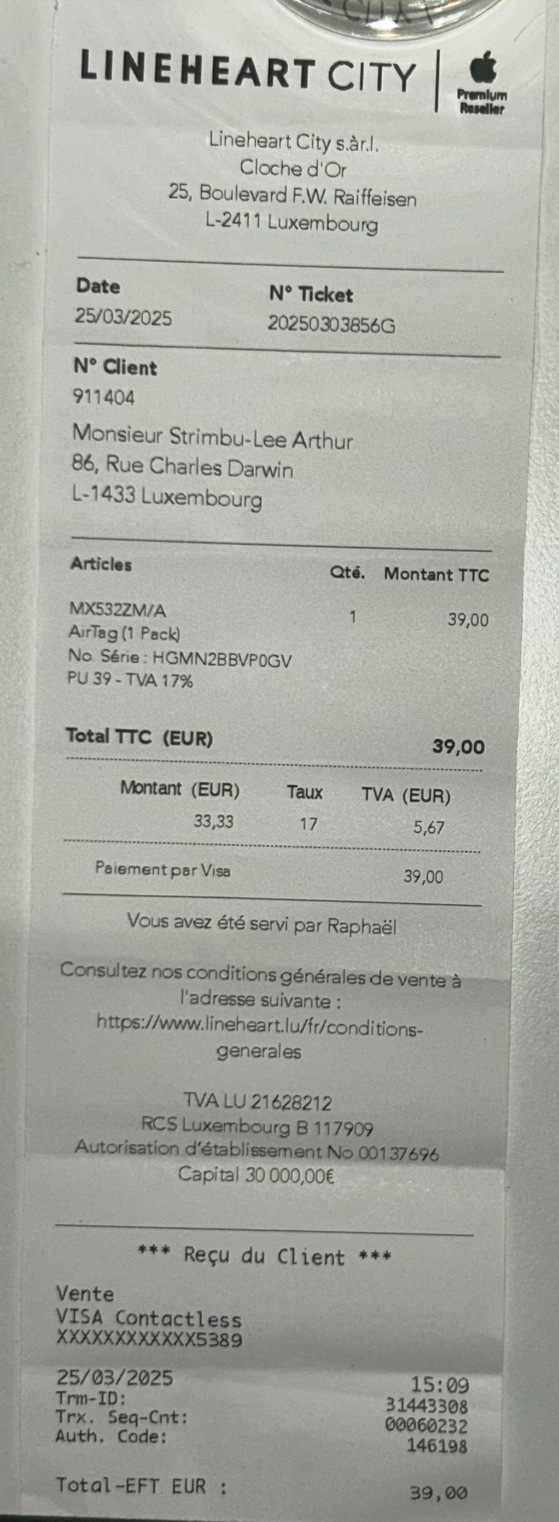
\includegraphics[width=0.3\textwidth]{images/Ticket de caisse.png} 
    \caption{AirTag receipt}
\end{figure}

\subsection{Outreach}

We posted quite regularly on the instagram account (Figure 16) and we  managed to grow it to 138 followers.
However, we did not have a lot of time to create the tutorial because of school and many other 
competitions. Nonetheless, we are still motivated to record the tutorial video. Our strategy is 
to involve our followers as much as possible. We make funny content and often ask question under 
the form of a poll for example. Recently, we asked them for marbles for our ball bearing system. In
counterpart, they will have their name on our Can. 

\begin{figure}[h] 
    \centering
    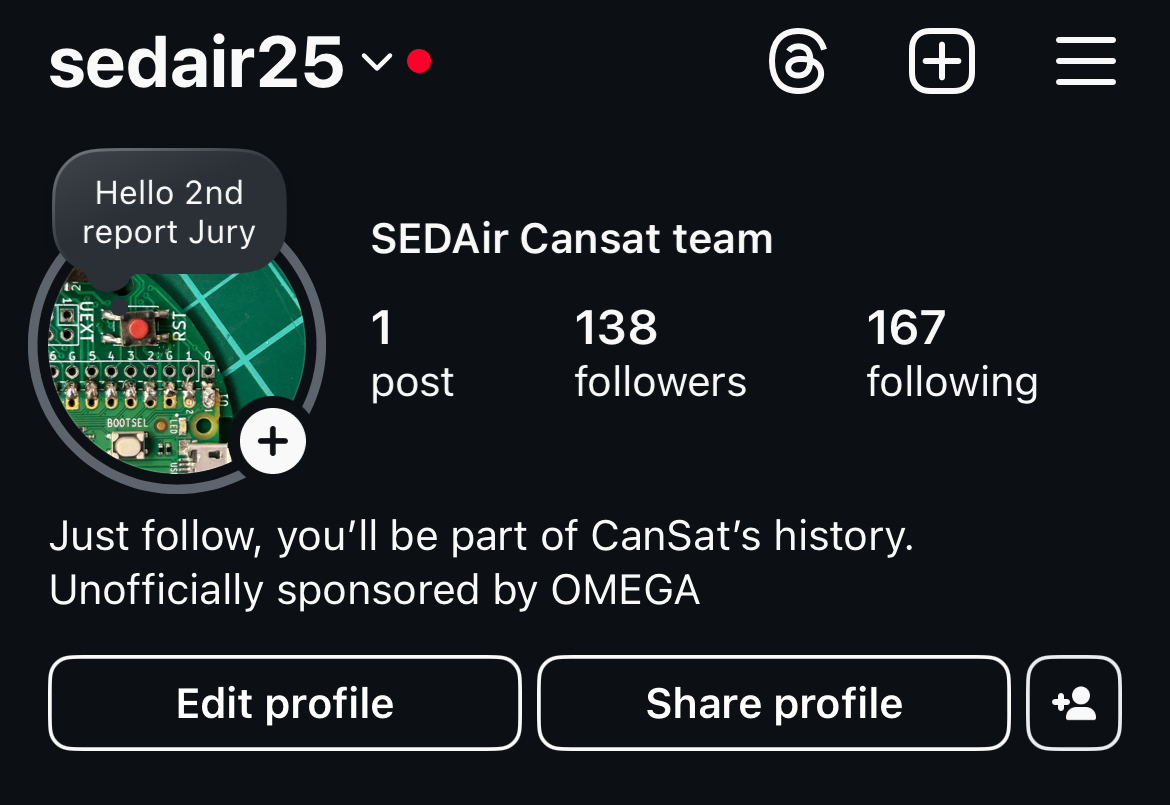
\includegraphics[width=0.5\textwidth]{images/Screen_instaaccount.jpg} 
    \caption{Our instagram account (don't forget to follow !)}
\end{figure}

We are quite famous in our school now (whithout arrogance) as we are considered "seniors" of CanSat. 
Therefore many teams in Vauban come to see us and ask for help and advice. This is a great way to
adverstise at a school level. The idea of a partneship is good, but it requires a lot of time and as
it is not crucial, we will not find a partneship with other science enthusiasts. 




%5 Scientific results
\section{Scientific results}

No launch, no results (coming soon ! we hope...)



%6 Discussion
\section{Discussion}

We are still rather confident so far.


%7 Conclusion
\section{Conclusion}

To conclude, we have made significant progress and are approaching the final stages of our project.

The primary mission is almost complete, with only a few adjustments and improvements remaining. The essential components are in place, and we are now refining the details.

Regarding the secondary mission, the prototypes for both the vertical and horizontal axes are finished, but the final project still requires completion, along with essential testing to validate its performance.

For the can, there is still considerable work to optimize its design, particularly regarding modifications to the closing system to enhance efficiency.

Concerning the antenna, the RSSI values remain too low, so we need to improve the signal strength either through coding adjustments or by implementing a new antenna.

The recovery system is fully developed, but further testing is required to analyze its performance and determine whether any improvements are necessary.

Finally, we aim to launch a new secondary mission incorporating additional sensors and algorithms.















\end{document}
